% ******************************* PhD Thesis Template **************************
% Please have a look at the README.md file for info on how to use the template

\documentclass[oneside,a4paper,12pt,bookman,numbered,print,index]{Classes/CSEThesisPSnPDF}
\usepackage{booktabs}
%\usepackage[utf8]{inputenc} % This for vietnamese 
%\usepackage[utf8]{vietnam} % This for vietnamese 

% ******************************************************************************
% ******************************* Class Options ********************************
% *********************** See README for more details **************************
% ******************************************************************************

% `a4paper'(The University of Cambridge PhD thesis guidelines recommends a page
% size a4 - default option) or `a5paper': A5 Paper size is also allowed as per
% the Cambridge University Engineering Deparment guidelines for PhD thesis
%
% `11pt' or `12pt'(default): Font Size 10pt is NOT recommended by the University
% guidelines
%
% `oneside' or `twoside'(default): Printing double side (twoside) or single
% side.
%	
% `print': Use `print' for print version with appropriate margins and page
% layout. Leaving the options field blank will activate Online version.
%
% `index': For index at the end of the thesis
%
% `draftclassic': For draft mode without loading any images (same as draft in book)
%
% `draft': Special draft mode with line numbers, images, and water mark with
% timestamp and custom text. Position of the text can also be modified.
%
% `abstract': To generate only the title page and abstract page with
% dissertation title and name, to submit to the Student Registry
%
% `chapter`: This option enables only the specified chapter and it's references
%  Useful for review and corrections.
%
% ************************* Custom Page Margins ********************************
%
% `custommargin`: Use `custommargin' in options to activate custom page margins,
% which can be defined in the preamble.tex. Custom margin will override
% print/online margin setup.
%
% *********************** Choosing the Fonts in Class Options ******************
%
% `times' : Times font with math support. (The Cambridge University guidelines
% recommend using times)
%
% `fourier': Utopia Font with Fourier Math font (Font has to be installed)
%            It's a free font.
%
% `customfont': Use `customfont' option in the document class and load the
% package in the preamble.tex
%
% default or leave empty: `Latin Modern' font will be loaded.
%
% ********************** Choosing the Bibliography style ***********************
%
% `authoryear': For author-year citation eg., Krishna (2013)
%
% `numbered': (Default Option) For numbered and sorted citation e.g., [1,5,2]
%
% `custombib': Define your own bibliography style in the `preamble.tex' file.
%              `\RequirePackage[square, sort, numbers, authoryear]{natbib}'.
%              This can be also used to load biblatex instead of natbib
%              (See Preamble)
%
% **************************** Choosing the Page Style *************************
%
% `default (leave empty)': For Page Numbers in Header (Left Even, Right Odd) and
% Chapter Name in Header (Right Even) and Section Name (Left Odd). Blank Footer.
%
% `PageStyleI': Chapter Name next & Page Number on Even Side (Left Even).
% Section Name & Page Number in Header on Odd Side (Right Odd). Footer is empty.
%
% `PageStyleII': Chapter Name on Even Side (Left Even) in Header. Section Number
% and Section Name in Header on Odd Side (Right Odd). Page numbering in footer


% ********************************** Preamble **********************************
% Preamble: Contains packages and user-defined commands and settings
% ******************************************************************************
% ****************************** Custom Margin *********************************

% Add `custommargin' in the document class options to use this section
% Set {innerside margin / outerside margin / topmargin / bottom margin}  and
% other page dimensions
\ifsetCustomMargin
  \RequirePackage[left=30mm,right=30mm,top=35mm,bottom=30mm]{geometry}
  \setFancyHdr % To apply fancy header after geometry package is loaded
\fi

\usepackage{listings}
\usepackage{color}
\definecolor{lightgray}{rgb}{.9,.9,.9}
\definecolor{darkgray}{rgb}{.4,.4,.4}
\definecolor{purple}{rgb}{0.65, 0.12, 0.82}
\usepackage{float}
\lstdefinelanguage{JavaScript}{
	keywords={typeof, new, true, false, catch, function, return, null, catch, switch, var, if, in, while, do, else, case, break},
	keywordstyle=\color{blue}\bfseries,
	ndkeywords={class, export, boolean, throw, implements, import, this},
	ndkeywordstyle=\color{darkgray}\bfseries,
	identifierstyle=\color{black},
	sensitive=false,
	comment=[l]{//},
	morecomment=[s]{/*}{*/},
	commentstyle=\color{purple}\ttfamily,
	stringstyle=\color{red}\ttfamily,
	morestring=[b]',
	morestring=[b]"
}

\lstset{
	language=JavaScript,
	backgroundcolor=\color{lightgray},
	extendedchars=true,
	basicstyle=\footnotesize\ttfamily,
	showstringspaces=false,
	showspaces=false,
	numbers=left,
	numberstyle=\footnotesize,
	numbersep=9pt,
	tabsize=2,
	breaklines=true,
	showtabs=false,
	captionpos=b
}




% Add spaces between paragraphs
%\setlength{\parskip}{0.5em}
% Ragged bottom avoids extra whitespaces between paragraphs
\raggedbottom
% To remove the excess top spacing for enumeration, list and description
%\usepackage{enumitem}
%\setlist[enumerate,itemize,description]{topsep=0em}

% *****************************************************************************
% ******************* Fonts (like different typewriter fonts etc.)*************

% Add `customfont' in the document class option to use this section

\ifsetCustomFont
  % Set your custom font here and use `customfont' in options. Leave empty to
  % load computer modern font (default LaTeX font).
  %\RequirePackage{helvet}

  % For use with XeLaTeX
  %  \setmainfont[
  %    Path              = ./libertine/opentype/,
  %    Extension         = .otf,
  %    UprightFont = LinLibertine_R,
  %    BoldFont = LinLibertine_RZ, % Linux Libertine O Regular Semibold
  %    ItalicFont = LinLibertine_RI,
  %    BoldItalicFont = LinLibertine_RZI, % Linux Libertine O Regular Semibold Italic
  %  ]
  %  {libertine}
  %  % load font from system font
  %  \newfontfamily\libertinesystemfont{Linux Libertine O}
\fi

% *****************************************************************************
% **************************** Custom Packages ********************************

% ************************* Algorithms and Pseudocode **************************

%\usepackage{algpseudocode}


% ********************Captions and Hyperreferencing / URL **********************

% Captions: This makes captions of figures use a boldfaced small font.
%\RequirePackage[small,bf]{caption}

\RequirePackage[labelsep=space,tableposition=top]{caption}
\renewcommand{\figurename}{Fig.} %to support older versions of captions.sty


% *************************** Graphics and figures *****************************

%\usepackage{rotating}
%\usepackage{wrapfig}

% Uncomment the following two lines to force Latex to place the figure.
% Use [H] when including graphics. Note 'H' instead of 'h'
%\usepackage{float}
%\restylefloat{figure}

% Subcaption package is also available in the sty folder you can use that by
% uncommenting the following line
% This is for people stuck with older versions of texlive
%\usepackage{sty/caption/subcaption}
\usepackage{subcaption}

% ********************************** Tables ************************************
\usepackage{booktabs} % For professional looking tables
\usepackage{multirow}

%\usepackage{multicol}
%\usepackage{longtable}
%\usepackage{tabularx}


% *********************************** SI Units *********************************
\usepackage{siunitx} % use this package module for SI units


% ******************************* Line Spacing *********************************

% Choose linespacing as appropriate. Default is one-half line spacing as per the
% University guidelines

%\doublespacing
%\onehalfspacing
%\singlespacing


% ************************ Formatting / Footnote *******************************

% Don't break enumeration (etc.) across pages in an ugly manner (default 10000)
%\clubpenalty=500
%\widowpenalty=500

%\usepackage[perpage]{footmisc} %Range of footnote options


% *****************************************************************************
% *************************** Bibliography  and References ********************

%\usepackage{cleveref} %Referencing without need to explicitly state fig /table

% Add `custombib' in the document class option to use this section
\ifuseCustomBib
   \RequirePackage[square, sort, numbers, authoryear]{natbib} % CustomBib

% If you would like to use biblatex for your reference management, as opposed to the default `natbibpackage` pass the option `custombib` in the document class. Comment out the previous line to make sure you don't load the natbib package. Uncomment the following lines and specify the location of references.bib file

%\RequirePackage[backend=biber, style=numeric-comp, citestyle=numeric, sorting=nty, natbib=true]{biblatex}
%\bibliography{References/references} %Location of references.bib only for biblatex

\fi

% changes the default name `Bibliography` -> `References'
\renewcommand{\bibname}{References}


% ******************************************************************************
% ************************* User Defined Commands ******************************
% ******************************************************************************

% *********** To change the name of Table of Contents / LOF and LOT ************

%\renewcommand{\contentsname}{My Table of Contents}
%\renewcommand{\listfigurename}{My List of Figures}
%\renewcommand{\listtablename}{My List of Tables}


% ********************** TOC depth and numbering depth *************************

\setcounter{secnumdepth}{3}
\setcounter{tocdepth}{2}


% ******************************* Nomenclature *********************************

% To change the name of the Nomenclature section, uncomment the following line

%\renewcommand{\nomname}{Symbols}


% ********************************* Appendix ***********************************

% The default value of both \appendixtocname and \appendixpagename is `Appendices'. These names can all be changed via:

%\renewcommand{\appendixtocname}{List of appendices}
%\renewcommand{\appendixname}{Appndx}
%\renewcommand{\appendixtocname}{List of appendices}
%\renewcommand{\appendixname}{Phụ lục}


% *********************** Configure Draft Mode **********************************

% Uncomment to disable figures in `draft'
%\setkeys{Gin}{draft=true}  % set draft to false to enable figures in `draft'

% These options are active only during the draft mode
% Default text is "Draft"
%\SetDraftText{DRAFT}

% Default Watermark location is top. Location (top/bottom)
%\SetDraftWMPosition{bottom}

% Draft Version - default is v1.0
%\SetDraftVersion{v1.1}

% Draft Text grayscale value (should be between 0-black and 1-white)
% Default value is 0.75
%\SetDraftGrayScale{0.8}


% ******************************** Todo Notes **********************************
%% Uncomment the following lines to have todonotes.

%\ifsetDraft
%	\usepackage[colorinlistoftodos]{todonotes}
%	\newcommand{\mynote}[1]{\todo[author=kks32,size=\small,inline,color=green!40]{#1}}
%\else
%	\newcommand{\mynote}[1]{}
%	\newcommand{\listoftodos}{}
%\fi

% Example todo: \mynote{Hey! I have a note}


% ************************ Thesis Information & Meta-data **********************
% Thesis title and author information, refernce file for biblatex
% ************************ Thesis Information & Meta-data **********************
%% The title of the thesis
\singlespacing \title{Ứng dụng Internet of Things để phát triển hệ thống thu thập và giám sát khí thải của phương tiện giao thông}
%\texorpdfstring is used for PDF metadata. Usage:
%\texorpdfstring{LaTeX_Version}{PDF Version (non-latex)} eg.,
%\texorpdfstring{$sigma$}{sigma}

%% Subtitle (Optional)
%\part{title}\subtitle{Using the CUED template}

%% University and Crest
%\university{HO CHI MINH CITY UNIVERSITY OF TECHNOLOGY}
\university{ĐẠI HỌC QUỐC GIA THÀNH PHỐ CHÍ MINH\\TRƯỜNG ĐẠI HỌC BÁCH KHOA}
%% Department (eg. Department of Engineering, Maths, Physics)
%\dept{FACULTY OF COMPUTER SCIENCE AND ENGINEERING}
\dept{KHOA KHOA HỌC VÀ KỸ THUẬT MÁY TÍNH}

% Crest minimum should be 30mm.
\crest{
\includegraphics[width=0.2\textwidth]{bklogo}}
%% Use this crest, if you are using the college crest

%% Crest long miminum should be 65mm
%\crest{
\includegraphics[width=0.45\textwidth]{University_Crest_Long}}

%% College shield [optional] 
% Crest minimum should be 30mm.
%\collegeshield{
\includegraphics[width=0.2\textwidth]{CollegeShields/Kings}}


%% Supervisor (optional)
%% for multiple supervisors, append each supervisor with the \newline command
\supervisor{\textbf{TS. Phạm Hoàng Anh}}
%\newline
%Prof. C.D. Supervisor\newline
%Prof. E.F. Supervisor\newline
%Prof. G.H. Supervisor}}

%% Supervisor Role (optional) - Supervisor (default) or advisor
%\supervisorrole{\textbf{Giảng viên hướng dẫn}}
\supervisorrole{{Giảng viên hướng dẫn:}}
%% if no title is desired:
% \supervisorrole{}

%% Advisor (optional)
%% for multiple advisors, append each advisor with the \newline command
%\advisor{Advisor 1\newline
%Advisors 2\newline
%Advisor 3\newline
%Advisor 4}
     
%% Advisor Role (optional) - Advisor (default) or leave empty
% \advisorrole{Advisors: }
%% if no title is required
% \advisorrole{}

%% The full name of the author
\author{	5120000 - Nguyễn Tấn Tùng\newline
		51202655 - Huỳnh Phạm So Ny\newline
		51200000 - Nguyễn Mạnh Cường}
\authorrole{Sinh viên thực hiện:}

%% You can redefine the submission text:
% Default as per the University guidelines:
% ``This dissertation is submitted for the degree of''
%\renewcommand{\submissiontext}{change the default text here if needed}

%% Full title of the Degree
\degreetitle{Ngành Kỹ Thuật Máy Tính}

%% College affiliation (optional)
%\college{King's College}

%% Submission date 
% Default is set as {\monthname[\the\month]\space\the\year}
\degreedate{Tháng 12 Năm 2016} 

%% Meta information
\subject{LaTeX} \keywords{{LaTeX} {Thesis} {Computer Engineering}}


% ***************************** Abstract Separate ******************************
% To printout only the titlepage and the abstract with the PhD title and the
% author name for submission to the Student Registry, use the `abstract' option in
% the document class.

%\ifdefineAbstract
% \pagestyle{empty}
% \includeonly{Declaration/declaration, Abstract/abstract}
%\fi

% ***************************** Chapter Mode ***********************************
% The chapter mode allows user to only print particular chapters with references
% Title, Contents, Frontmatter are disabled by default
% Useful option to review a particular chapter or to send it to supervisior.
% To use choose `chapter' option in the document class

%\ifdefineChapter
% \includeonly{Chapter3/chapter3}
%\fi

% ******************************** Front Matter ********************************
\begin{document}

\frontmatter
\maketitle

\doublespacing
%% ******************************* Thesis Dedidcation ********************************

\begin{dedication} 

I would like to dedicate this thesis to my loving parents \dots

\end{dedication}


% ******************************* Thesis Declaration ***************************

\begin{declaration}

I hereby declare that except where specific reference is made to the work of 
others, the contents of this dissertation are original and have not been 
submitted in whole or in part for consideration for any other degree or 
qualification in this, or any other university. This dissertation is my own 
work and contains nothing which is the outcome of work done in collaboration 
with others, except as specified in the text and Acknowledgements. This 
dissertation contains fewer than 65,000 words including appendices, 
bibliography, footnotes, tables and equations and has fewer than 150 figures.

% Author and date will be inserted automatically from thesis.tex \author \degreedate

\end{declaration}


% ************************** Thesis Acknowledgements **************************

\begin{acknowledgements}
\title{Lời Cảm ơn}      

	Em xin gởi lời cảm ơn chân thành và sự tri ân sâu sắc đối với các thầy cô của trường Đại học Bách Khoa thành phố Hồ Chí Minh, đặc biệt là các thầy cô khoa Khoa Học và Kỹ Thuật Máy Tính của trường đã tạo điều kiện cho em thực tập ở khoa để có nhiều thời gian cho luận văn tốt nghiệp. Đặc biệt, xin gửi lời cám ơn chân thành Tiến sĩ Phạm Hoàng Anh đã nhiệt tình hướng dẫn hướng dẫn hoàn thành tốt đợt thực tập. Cám ơn các bạn Nguyễn Thị Trang 91103730, Đỗ Thành Nhân G1302688 đã có những đóng góp quý báu cùng với nhóm.

Trong quá trình thực tập, cũng như là trong quá trình làm bài báo cáo, khó tránh khỏi sai sót, rất mong các Thầy, Cô bỏ qua. Đồng thời do trình độ lý luận cũng như kinh nghiệm thực tiễn còn hạn chế nên bài báo cáo không thể tránh khỏi những thiếu sót, em rất mong nhận được ý kiến đóng góp Thầy, Cô để em học thêm được nhiều kinh nghiệm và sẽ hoàn thành tốt hơn bài luận văn sắp tới.
Em xin chân thành cảm ơn!

\begin{flushright}
Nhóm thực hiện đề tài.
\end{flushright} 



\end{acknowledgements}

% ************************** Thesis Abstract *****************************
% Use `abstract' as an option in the document class to print only the titlepage and the abstract.
\begin{abstract}
\renewcommand{\abstractname}{Tóm Tắt}

Do nhu cầu áp dụng khoa học và kỹ thuật vào phát triển hệ thống giám sát môi trường và giao thông, sinh viên nhóm chúng tôi đã tìm hiểu và thực hiện dự án hệ thống thu thập tình trạng ô nhiễm do khí thải của các phương tiện giao thông. Nhờ sự phát triển mạnh mẽ của Internet of Things, đề tài được định hướng phát triển theo mô hình IoT kết hợp với các kiến thức về môi trường nhằm để xây dụng hệ thống thiết bị đo đạc và lấy dữ liệu để phân tích. Nhóm bắt đầu tìm hiểu về các loại khí thải của phương tiện giao thông, tìm hiểu các cảm biến, các loại vi xử lý hỗ trợ tốt cho hệ thống IoT, kết hợp với hệ thống Cloud Database và ứng dụng Web theo dõi tình trạng ô nhiễm thực tế trên một số đoạn đường đã được đo đạc.

\end{abstract}


% *********************** Adding TOC and List of Figures ***********************
\onehalfspacing
\tableofcontents
\listoffigures
\listoftables

 %\printnomenclature[space] space can be set as 2em between symbol and description
%\printnomenclature[2em]
\doublespacing
\printnomenclature

% ******************************** Main Matter *********************************
\mainmatter

%*******************************************************************************
%*********************************** First Chapter *****************************
%*******************************************************************************

\chapter{Giới thiệu}  %Title of the First Chapter

\ifpdf
    \graphicspath{{Chapter1/Figs/Raster/}{Chapter1/Figs/PDF/}{Chapter1/Figs/}}
\else
    \graphicspath{{Chapter1/Figs/Vector/}{Chapter1/Figs/}}
\fi


%********************************** %First Section  **************************************
\section{Ý tưởng và tính cấp thiết của đề tài} %Section - 1.1 
\label{section1.1}

Ngày nay, bài toán giao thông vẫn đang là bài toán hóc búa vẫn chưa được giải quyết được ở Việt Nam và nhiều nước đang phát triển. Tình trạng kẹt xe, ùn tắc kéo dài gây ra sự chậm trễ trong công việc, hơn nữa còn  gây gia tăng ô nhiễm môi trường, giảm chất lượng môi trường sống. Một trong những khó khăn làm bài toán giao thông khó giải quyết đó chính là không có đầy đủ dữ liệu cần thiết. Chúng ta không thể giải bài toán nếu không có đủ dữ kiện, cũng như giải quyết kẹt xe ta cần phải có dữ liệu về lưu lượng giao thông.

Vì yếu tố trên, dự án Smart Traffic được hình thành và phát triển theo hướng IoT với mục đích thu thập dữ liệu về các yếu tố môi trường (nồng độ CO, nhiệt độ, độ ẩm, nồng độ bụi, độ ồn…) và xác định mối tương quan giữa lưu lượng giao thông với môi trường xung quanh khu vực đó. Từ đó ta có thể có được 1 phần dữ liệu cần thiết về tình trạng các con đường theo thời gian thực, cũng như có được lịch sử và dùng dữ liệu ấy để phát triển dự đoán tình trạng giao thông tiếp theo.

\begin{figure}[htbp!] 
\centering    
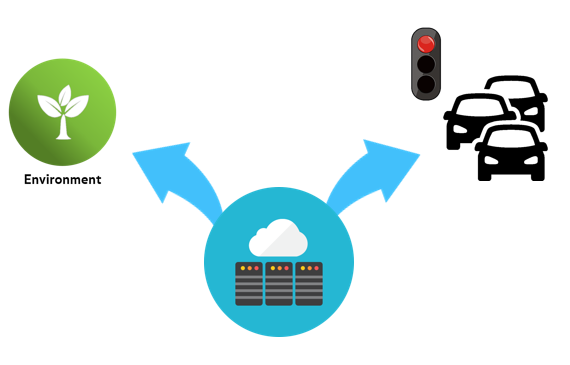
\includegraphics[width=1.0\textwidth]{pic1}
\caption[Mo hinh IoT ]{Mo ta tam hinh Mo hinh IoT}
\label{fig:pic1}
\end{figure}

Những dữ liệu đó có thể được phân tích và xử lý, đưa ra những kết luận về tình trạng lưu thông trên đoạn đường đó, về sự thay đổi môi trường tại 1 khu vực ở những khoảng thời gian khác nhau. Và những dữ liệu này có thể ứng dụng cho bất động sản, môi trường và nghiên cứu. Do đó đề tài mang tính thiết thực và ứng dụng cao và được lựa chọn để làm Thực tập tốt nghiệp và có thể lên Luận văn tốt nghiệp.




\section{Mục tiêu và nhiệm vụ của đề tài} %Section - 1.1 
\label{section1.2}
\subsection{Mục tiêu đề tài}
\begin{itemize}
\item[-]Tìm hiểu về khí thải xe máy và ô tô.

\item[-]Hiện thực mạch cảm biến để thu thập khí thải.

\item[-]Khảo sát và đo khí thải thực tế tại một số điểm thường xuyên xảy ra kẹt xe trên địa bàn thành phố.

\item[-]Tổng hợp các số liệu thu thập và các yếu tố môi trường khác (nhiệt độ, độ ẩm, …) để đề xuất mô hình để hướng đến phát triển hệ thống cảnh báo kẹt xe dựa vào tình trạng ô nhiễm không khí.




\end{itemize}

\subsection{Nhiệm vụ đề tài}
Phân chia công việc tại đây!!!! Sony, Tùng, Cường làm nhừng gì, vẽ giản đồ gantt.



%*******************************************************************************
%****************************** Second Chapter *********************************
%*******************************************************************************

\chapter{IoT và Các kiến thức cơ bản về IoT}

\ifpdf
    \graphicspath{{Chapter2/Figs/Raster/}{Chapter2/Figs/PDF/}{Chapter2/Figs/}{Chapter2/Figs/web/}}
\else
    \graphicspath{{Chapter2/Figs/Vector/}{Chapter2/Figs/}}
\fi


%\section[Short title]{Reasonably long section title}
\section{Giới thiệu về Internet of Things và các ứng dụng giám sát}
\subsection{Internet of Things (IoT)}
Với sự phát triển nhanh chóng của công nghê máy tính hiện nay, những công nghệ cao đã đang và ngày càng được ứng dụng trong nhiều lĩnh vực của cuộc sống con người. IoT là mạng lưới của các đối tượng vật lý, các thiết bị, các phương tiện và các đối tượng này được nhúng với các thiết bị điện tử, cảm biến, phần mềm điều khiển, và nó có khả năng trao đổi dữ liệu và thao tác với nhau. IoT cho phép các đối tượng được lắng nghe và điều khiển từ xa trên cơ sở hạ tầng mạng hiện có, các hệ thống máy tính có thể thu thập dữ liệu và điều khiển các thiết bị đối tượng một cách hiệu quả, chính xác và lợi ích kinh tế nhất có thể. 
\begin{figure}[htbp!] 
\centering    
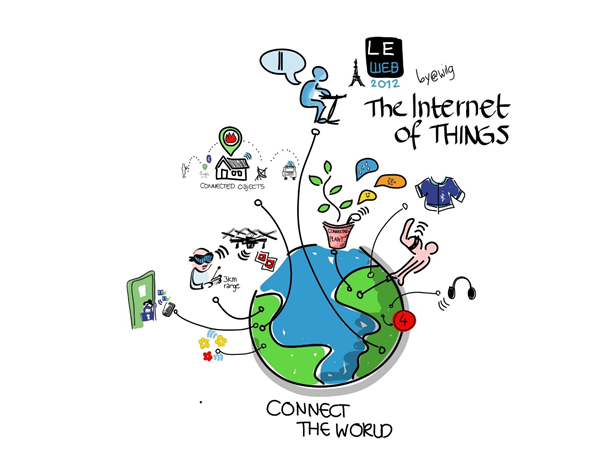
\includegraphics[width=1.0\textwidth]{pic4}
\caption[Hình ảnh mô tả Internet of Things ]{Hình ảnh mô tả Internet of Things }
\label{fig:pic4}
\end{figure}


\subsection*{Khả năng định danh độc nhất }
Điểm quan trọng của IoT đó là các đối tượng phải có thể được nhận biết và định dạng. Nếu mọi đội tượng, kể cả con người, được "đánh dấu" để phân biệt bản thân đối tượng đó với những thứ xung quanh thì chúng ta có thể hoàn toàn quản lí được nó thông qua máy tính. Việc đánh dấu có thể được thực hiện thông qua nhiều công nghệ, chẳng hạn như RFID, NFC, mã vạch, mã QR, watermark kĩ thuật số... Việc kết nối thì có thể thực hiện qua Wi-Fi, mạng viễn thông băng rộng (3G, 4G), Bluetooth, ZigBee, hồng ngoại...
Ngoài những kĩ thuật nói trên, nếu nhìn từ thế giới web, chúng ta có thể sử dụng các địa chỉ độc nhất để xác định từng vật, chẳng hạn như địa chỉ IP. Mỗi thiết bị sẽ có một IP riêng biệt không nhầm lẫn. Sự xuất hiện của IPv6 với không gian địa chỉ cực kì rộng lớn sẽ giúp mọi thứ có thể dễ dàng kết nối vào Internet cũng như kết nối với nhau.

\subsection*{Xu hướng và tính chất của The Internet of Things }
\textbf{Thông minh:} Sự thông minh và tự động trong điều khiển thực chất không phải là một phần trong ý tưởng về IoT. Các máy móc có thể dễ dàng nhận biết và phản hồi lại môi trường xung quanh (ambient intelligence), chúng cũng có thể tự điều khiển bản thân (autonomous control) mà không cần đến kết nối mạng. Tuy nhiên, trong thời gian gần đây người ta bắt đầu nghiên cứu kết hợp hai khái niệm IoT và autonomous control lại với nhau. Tương lai của IoT có thể là một mạng lưới các thực thể thông minh có khả năng tự tổ chức và hoạt động riêng lẻ tùy theo tình huống, môi trường, đồng thời chúng cũng có thể liên lạc với nhau để trao đổi thông tin, dữ liệu.

Việc tích hợp trí thông minh vào IoT còn có thể giúp các thiết bị, máy móc, phần mềm thu thập và phân tích các dấu vết điện tử của con người khi chúng ta tương tác với những thứ thông minh, từ đó phát hiện ra các tri thức mới liên quan tới cuộc sống, môi trường, các mối tương tác xã hội cũng như hành vi con người.

\textbf{Kiến trúc dựa trên sự kiện:} Các thực thể, máy móc trong IoT sẽ phản hồi dựa theo các sự kiện diễn ra trong lúc chúng hoạt động theo thời gian thực. Một số nhà nghiên cứu từng nói rằng một mạng lưới các sensor chính là một thành phần đơn giản của IoT.

\textbf{Là một hệ thống phức tạp:}Trong một thế giới mở, IoT sẽ mang tính chất phức tạp bởi nó bao gồm một lượng lớn các đường liên kết giữa những thiết bị, máy móc, dịch vụ với nhau, ngoài ra còn bởi khả năng thêm vào các nhân tốc mới.

\textbf{Kích thước: } Một mạng lưới IoT có thể chứa đến 50 đến 100 nghìn tỉ đối tượng được kết nối và mạng lưới này có thể theo dõi sự di chuyển của từng đối tượng. Một con người sống trong thành thị có thể bị bao bọc xung quanh bởi 1000 đến 5000 đối tượng có khả năng theo dõi.

\textbf{Vấn đề không gian, thời gian: }Trong IoT, vị trí địa lý chính xác của một vật nào đó là rất quan trọng. Hiện nay, Internet chủ yếu được sử dụng để quản lí thông tin được xử lý bởi con người. Do đó những thông tin như địa điểm, thời gian, không gian của đối tượng không mấy quan trọng bởi người xử lí thông tin có thể quyết định các thông tin này có cần thiết hay không, và nếu cần thì họ có thể bổ sung thêm. Trong khi đó, IoT về lý thuyết sẽ thu thập rất nhiều dữ liệu, trong đó có thể có dữ liệu thừa về địa điểm, và việc xử lí dữ liệu đó được xem như không hiệu quả. Ngoài ra, việc xử lí một khối lượng lớn dữ liệu trong thời gian ngắn đủ để đáp ứng cho hoạt động của các đối tượng cũng là một thác thức hiện nay.

\newpage

\subsection*{Mô hình theo xu hướng IoT thực tế}
Mô hình (Hình ~\ref{fig:pic5}): Các thiết bị sẽ có thể kết nối với nhau bằng TCP/UDP và có thể kết nối trực tiếp đến máy chủ mà không cần thông qua thiết bị khác.

\begin{figure}[htbp!] 
\centering    
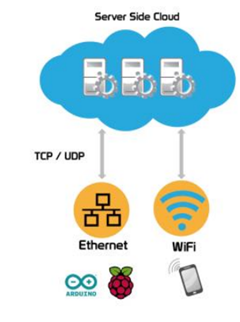
\includegraphics[width=0.5\textwidth]{pic5}
\caption[Mô hình IoT không có Gateway ]{Mô hình IoT không có Gateway}
\label{fig:pic5}
\end{figure}

Mô hình (Hình ~\ref{fig:pic6}): Các thiết bị sẽ được hỗ trợ nhiều chuẩn giao tiếp khác nhau (BLE, ZWave,…) nên cần cầu nối là Gateway để kết nối đến máy chủ. 
	
	

\begin{figure}[htbp!] 
\centering    
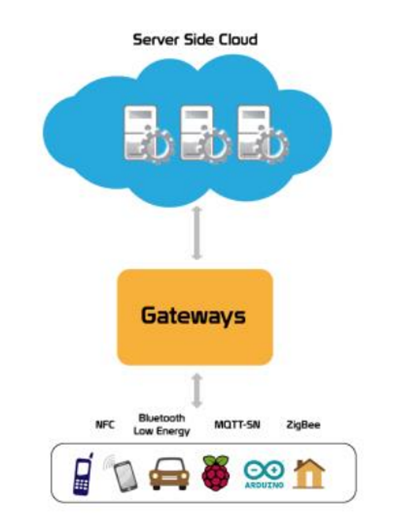
\includegraphics[width=0.5\textwidth]{pic6}
\caption[Mô hình IoT có Gateway]{Mô hình IoT có Gateway}
\label{fig:pic6}
\end{figure}


Sơ đồ lớp Chung của cả hai mô hình trên:


\begin{figure}[htbp!] 
\centering    
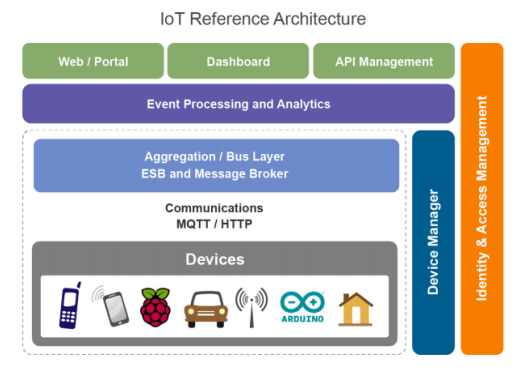
\includegraphics[width=1\textwidth]{pic7}
\caption[Kiến trúc mô hình IoT tham khảo]{Kiến trúc mô hình IoT tham khảo}
\label{fig:pic7}
\end{figure}



\begin{itemize}
\item[•]Lớp Device \\
Lớp dưới cùng của kiến trúc là lớp thiết bị. Thiết bị có thể được các loại khác nhau, nhưng để có thể được xem là thiết bị IOT, nó phải có một số thông tin liên lạc hoặc gián tiếp hoặc trực tiếp với Internet.\\
Mỗi thiết bị thường cần một ID. ID có thể là: Bluetooth identifier, Wi-Fi MAC Address…
\item[•]Lớp Communications \\
Các lớp truyền thông hỗ trợ các kết nối của các thiết bị tới máy chủ. Có nhiều giao thức để giao tiếp giữa các thiết bị và máy chủ. Nổi bật nhất là HTTP hoặc MQTT.\\
HTTP rất thông dụng. Bởi vì nó là một giao thức dựa trên văn bản đơn giản, nhiều thiết bị nhỏ như bộ điều khiển 8-bit có thể hỗ trợ một phần các giao thức - ví dụ đủ dữ liệu để POST hoặc GET một nguồn tài nguyên. Các thiết bị lớn hơn 32-bit có thể sử dụng đầy đủ các thư viện HTTP client đúng cách để hiện thực toàn bộ giao thức.\\
MQTT được phát minh vào năm 1999 để giải quyết các vấn đề trong hệ thống nhúng và SCADA. Nó đã được thông qua một số lần lặp lại và phiên bản hiện tại (3.1.1) đang trải qua những tiêu chuẩn hoá trong OASIS MQTT kỹ thuật Committee8. MQTT là một hệ thống tin nhắn publish-subscribe dựa trên một mô hình broker. Các giao thức có một chi phí rất nhỏ (ít nhất là 2 byte cho mỗi tin nhắn). MQTT được thiết kế để vận hành qua TCP.

\item[•]Lớp Aggregation/Bus \\
Một lớp quan trọng của kiến trúc là lớp mà tập hợp và là cầu nối, có khả năng tổng hợp và kết hợp các thông tin liên lạc từ các thiết bị khác nhau và đưa thông tin liên lạc đến một thiết bị cụ thể (có thể thông qua một gateway).
\item[•]Lớp Event Processing and Analytic: \\
Lớp này có các sự kiện từ lớp Bus và cung cấp khả năng xử lý và hành động theo những sự kiện này. Yêu cầu phải lưu trữ các dữ liệu vào một cơ sở dữ liệu nên buộc phải có một ứng dụng ở máy chủ.
\item[•]Lớp External Communications (Top) \\
Lớp này cung cấp một cách cho các thiết bị để chúng giao tiếp ra bên ngoài hệ thống một cách có định hướng và thân thiện với người dùng (Web, Dashboard, API Management)
\end{itemize}

% Please add the following required packages to your document preamble:

\begin{table}[]
\centering
\caption{My caption}
\label{my-label}
\begin{tabular}{|l|l|l|}
\hline
\textbf{MÔ HÌNH} & \textbf{ƯU ĐIỂM} & \textbf{NHƯỢC ĐIỂM} \\ \hline
\textbf{Mô hình cũ} & Đơn giản hiện thực & \begin{tabular}[c]{@{}l@{}}Gateway cồng kềnh vì phải có \\ bộ phận thu/phát hồng ngoại \\ và các mạch để giao tiếp RF.\end{tabular} \\ \hline
\textbf{Mô hình 1} & \begin{tabular}[c]{@{}l@{}}Không cần thông qua \\ gateway, mọi thông tin \\ thiết bị đều được lưu \\ trên máy chủ.\end{tabular} & \begin{tabular}[c]{@{}l@{}}Hạn chế về phương thức giao\\ tiếp vì chỉ sử dụng TCP/UDP \\ để giao tiếp. Không thể điều khiển\\  thiết bị khi không truy cập được \\ máy chủ.\end{tabular} \\ \hline
\textbf{Mô hình 2} & \begin{tabular}[c]{@{}l@{}}Quản lý thiết bị thông qua\\ gateway làm trung gian, nên\\ các thiết bị có thể tương tác\\ với nhau dễ dàng mà không \\ cần đến máy chủ.\end{tabular} & \begin{tabular}[c]{@{}l@{}}Chi phí cao hơn, hệ thống \\ phức tạp hơn. Độ bảo mật \\ cũng cần được quan tâm hơn.\end{tabular} \\ \hline
\end{tabular}
\end{table}



	
\subsection{Các hệ thống giám sát được phát triển dựa trên IoT}
Khi kết nối một chuỗi khổng lồ các cảm biến (sensor) thu thập dữ liệu, thiết bị và máy móc với nhau, điều quan trọng cần nhận ra là thông tin sẽ được chuyển đổi thành hành động với một tốc độ mà chúng ta chưa từng thấy trước kia. Chúng ta đang tiến đến gần, nếu không phải là đã chạm được vào một thế giới của những khoảng thời gian phản ứng cực nhỏ, phản hồi tức thì với mọi điều kiện biến đổi, và mức độ điều khiển chưa từng có trong việc quản lý tài nguyên và tài sản.
Điểm mấu chốt ở đây là đừng nghĩ hẹp. Internet of Things (IoT) không đơn thuần là mang đến sự tiết kiệm trong các mô hình công nghiệp hiện tại. Nó đảo lộn hoàn toàn những mô hình cũ, tạo ra những sản phẩm và dịch vụ mới. Không có một lĩnh vực nào mà trong đó IoT tạo ra ảnh hưởng đặc biệt lớn nhất; bởi IoT sẽ thay đổi hoàn toàn mọi lĩnh vực một cách không thể tưởng tượng được, bao gồm nông nghiệp, năng lượng, an ninh, quản lý thảm họa, y tế, và đó chỉ là một vài lĩnh vực được nhắc đến.

\subsection*{Ứng dụng trong xây dụng }
\begin{figure}[htbp!] 
\centering    

\includegraphics[width=1\textwidth]{pic8}
\caption[Ứng dụng IoT trong xây dựng ]{Ứng dụng IoT trong xây dựng }
\label{fig:pic8}
\end{figure}

Ví dụ: Các công ty xây dựng đã bắt đầu trang bị các silo (hầm chứa đồ) và xe tải có các cảm biến theo dõi mức hàng tồn kho, như là lượng bê tông, và biến đổi nó thông qua platform trên nền điện toán đám mây để gia tăng tốc độ phân phối và đảm bảo một dòng lưu thông vật liệu ổn định. Các ông lớn trong ngành công nghiệp dầu mỏ đã bắt đầu thực thi các công nghệ mobile, cảm biến tới máy móc để dự phòng từ trước cho các tai nạn thông qua các phân tích nhanh chóng và hành động tức thời. Khi các cảm biến phát hiện ra một sự cố như rò rỉ hoặc thất thoát đường ống, công nghệ IoT cho phép các công nhân lập tức xác định vị trí của chúng.

\subsection*{Ứng dụng trong năng lượng }

\begin{figure}[htbp!] 
\centering    
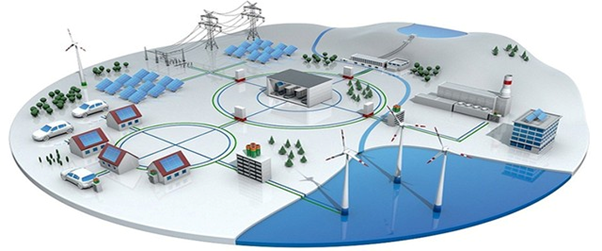
\includegraphics[width=1\textwidth]{pic9}
\caption[Ứng dụng IoT trong năng lượng]{Ứng dụng IoT trongnăng lượng}
\label{fig:pic9}
\end{figure}
Một ví dụ khác của công nghệ IoT mới ứng dụng trong công nghiệp dầu mỏ, đó là giếng thông minh. Đây là một dạng giếng cài đặt các thiết bị điều khiển dòng chảy và cảm biến lỗ khoan, để có thể giám sát và điều khiển từ trên bề mặt mà không đe dọa an toàn của công nhân. Giếng thông minh có trang bị công nghệ địa chấn 4D, cho phép theo dõi sự rò rỉ khí ga, dòng chảy nước, thay đổi áp lực, và bất cứ thay đổi nào khác gây ra bởi những biến động địa chấn, giúp cho việc dự đoán và điều khiển các tác động địa chấn có thể gây ra những hỏng hóc nghiêm trọng.
Nhưng như thế, chúng ta vẫn nghĩ quá hẹp. Hãy vượt ra khỏi lĩnh vực xây dựng hay năng lượng. Chúng ta có các cảm biến có thể đo lực, tải, moment, và áp lực; các cảm biến có thể ngửi thấy mùi khí ga hay hóa chất; những cảm biến có thể nghe thấy rung động và phân biệt giữa các âm hưởng khác nhau; những cảm biến có thể đo nhiệt độ, phát hiện chuyển động, vận tốc và chuyển vị; xác định vị trí, sự có mặt, và khoảng cách. Nói cách khác, chúng ta có khả năng thu thập những hiểu biết gần như không giới hạn, trong thời gian thực.

\subsection*{Ứng dụng trong dân dụng  }

\begin{figure}[htbp!] 
\centering    
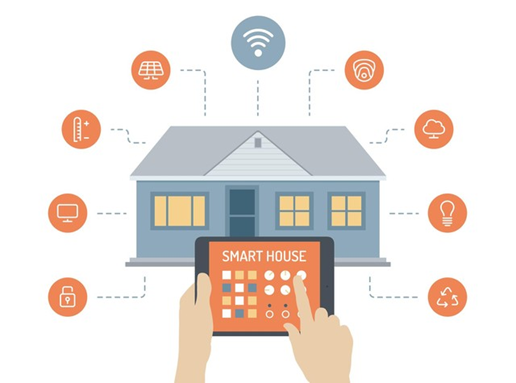
\includegraphics[width=1\textwidth]{pic10}
\caption[Ứng dụng IoT trong dân dụng ]{Ứng dụng IoT trong dân dụng}
\label{fig:pic10}
\end{figure}

Làm thế nào chúng ta có thể tận dụng thông tin thời gian thực từ rất nhiều sensor? Hãy nhìn vào ngôi nhà của chúng ta. Những phần nào trong đó có thể thông minh hóa? Ví dụ đơn giản. Tôi từng quan sát 1 hệ thống video conference cho phép người chủ nói chuyện với chú cún của mình, gọi nó đến, cho nó ăn từ xa thông qua một thiết bị thông minh. Hãy nghĩ lớn hơn nữa. Một ngôi nhà biết khi nào bạn về nhà bởi nó kết nối với một cảm biến trên xe hay smartphone của bạn. Một ngôi nhà kết nối các cảm biến báo khói, hệ thống an ninh, và thiết bị giải trí tới điện thoại của bạn. Một ngôi nhà với các cảm biến được gắn vào đường ống để có thể phát hiện ra rò rỉ trước cả khi điều đó thực sự diễn ra.

\subsection*{Ứng dụng trong y tế}
\begin{figure}[htbp!] 
\centering    
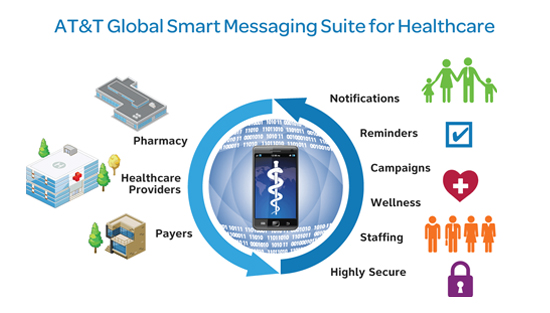
\includegraphics[width=1\textwidth]{pic11}
\caption[Ứng dụng IoT trong y tế ]{Ứng dụng IoT trong y tế}
\label{fig:pic11}
\end{figure}
Công nghệ thiết bị đeo cũng sẽ biến đổi hoàn toàn lĩnh vực chăm sóc sức khỏe theo những cách phi thường. Chúng ta đều biết rằng đồng hộ Apple Watch sẽ tích hợp một cảm biến theo dõi nhịp tim và cung cấp cho chủ của nó những ứng dụng tạo điều kiện và khuyến khích một cách sống lành mạnh. Chúng ta đã có các cảm biến gắn trong giày để theo dõi việc chạy xa đến đâu và bao nhiêu calo đã được đốt. Còn gì tiếp theo? Sẽ có một quy trình tối ưu chăm sóc sức khỏe, theo đó có những cảm biến có thể phát hiện vi khuẩn trong thiết bị, và thiết bị diệt khuẩn phát hiện virus có thể di chuyển từ bệnh nhân.


\section{Giới thiệu về các công cụ hỗ trợ phát triển ứng dụng IoT}




\section{Những yếu tố ảnh hưởng môi trường từ khí thải phương tiện giao thông}
Để hình dung được những yếu tố ảnh hưởng môi trường từ khí thải xe máy và ô tô thì chúng ta cần biết được quá trình hoạt động của xe máy và ô tô, từ đó chúng ta sẽ biết được những loại khí thải nào mà xe máy và ô tô sẽ thải ra môi trường. Qua quá trình tìm hiểu và đọc thông tin tài liệu trên mạng khí thải của xe máy và ô tô tuỳ thuộc chủ yếu vào chất lượng đốt cháy hỗn hợp xăng và không khí bên trong buồng đốt (combustion chamber) của động cơ, cũng như nồng độ các chất ô nhiễm trong khí xả phụ thuộc vào đặc điểm động cơ cũng như các thông số điều chỉnh, vận hành.

Động cơ mới và được điều chỉnh đúng cho phản ứng cháy hoàn chỉnh (complete combustion) hay phản ứng cháy thừa oxy:

\begin{center}
PTPU: Xăng + Không khí → Carbon Dioxide + Nước + Nitrogen
\end{center} 
Các phó sản (by-product) chủ yếu của phản ứng này là nước (H2O) và carbon dioxide (CO2), do đó ống thoát khí cháy (tail pipe) của một động cơ tốt thường có nước nhễu ra, dễ nhận thấy khi động cơ đang trong quá trình làm nóng máy (warm up).
Động cơ cũ hoặc không được điều chỉnh đúng cho phản ứng cháy không hoàn chỉnh (incomplete combustion) hay thiếu oxy:
\begin{center}
PTPU: Xăng + Không khí → Hydrocarbons + Nitrogen Oxides + Carbon Dioxide + Carbon Monoxide + Nước
\end{center}

Phản ứng này tạo thêm những phó sản như carbon monoxide (CO) và nitrogen oxides (NOx). Vậy chúng ta có các loại sản pham như sau:
\begin{itemize}
\item[•]CO được sinh ra khi lượng oxy đưa vào buồng đốt không đủ.
\item[•]HC được sinh ra trong quá trình đốt cháy không hoàn toàn, cũng như CO.
\item[•]NOx được sinh ra do nitơ và ôxy trong hỗn hợp không khí-nhiên liệu, khi nhiệt độ của buồng đốt tăng cao trên 1800oC.
\end{itemize}
 Nhiệt độ của buồng đốt càng cao, lượng NOx sản ra càng nhiều.
Theo lý thuyết, khi đốt cháy xăng thì chỉ sinh ra CO2 (cácbon điôxit) và H2O (hơi nước). Tuy nhiên, không phải toàn bộ xăng đều tham gia phản ứng như lí thuyết, do ảnh hưởng của các yếu tố như tỷ lệ hỗn hợp không khí-nhiên liệu, nitơ trong không khí, nhiệt độ cháy, thời gian cháy... Đó là nguyên nhân sinh ra các khí độc hại như CO, HC hoặc NOx.
Trên cơ sở thực tế, động cơ đốt trong nó chỉ sử dụng được khoảng 30-45\% nhiệt lượng để sinh công, phần còn lại bị hao hụt đi mất, do đó nó mang theo nhiệt lượng thải ra ngoài. Lượng nhiệt này thực tế đã tác động đến môi trường, làm cho nhiệt độ xung quanh những khu vực có xe máy và ô tô tăng lên. Việc đi lại trên những đoạn đường đông xe máy và ô tô thường gây cho chúng ta cảm giác nóng bức, và khó thở. Đó chính là những yếu tố khí thải đã trình bày như trên của xe máy và ô tô đã tác động đến môi trường.
Một phần nhân tố cũng đáng chú ý trong quá trình hoạt động xe máy và ô tô hoạt động đó là bụi, vì đầu vào của động cơ là xăng và không khí, mà trong xăng hiện nay thường có cặn và lượng không khí đầu vào cũng có bụi mặc dù có bộ lọc khí nhưng không thể tránh được trong quá trình sử dụng lâu dài. Một số loại phương tiện giao thông sử dụng thời gian dài, không đi bảo trì sẽ thải ra một nồng độ ô nhiễm rất lớn.
Từ những cơ sơ lý thuyết trên cho chúng ta biết được những yếu tố ảnh hưởng môi trường từ khí thải xe máy và ô tô bao gồm:
\begin{itemize}
\item[•]Khí CO2, CO, HC, NOx.
\item[•]Khói bụi.
\item[•]Yếu tố về nhiệt.
\end{itemize}








\section{Các hệ thống quan trắc hiện hữu}
\textbf{VoV giao thông:}  sử dụng hệ thống camera an ninh kết hợp với lượng phóng viên thường trực khắp thành phố để giám sát trực tiếp và cảnh báo tình trạng lưu thông trên các đoạn đường. Hệ thống có tính hiệu quả rất cao vì sử dụng CCTV giám sát tình trạng giao thông theo thời gian thực nên có góc nhìn thực tế nhất và không phục thuộc, có thể hoạt động độc lập. Tuy nhiên hệ thống vẫn có nhiều hạn chế như:
\begin{itemize}
\item[•]Vẫn chủ yếu hoạt động một cách thủ công, điều tiết và đưa ra kết quả bởi con người, chưa có áp dụng thuật toán xử lý máy tính vào công việc nhiều.
\item[•]Tốn nhiều công sức và nhân lực, cần có nhiều phóng viên trực thuộc các đoạn đường cũng như người quản lý theo dõi hệ thống camera giao thông.
\item[•]Chi phí duy trì và lắp đặt còn khá cao, và cần tốn chi phí bảo trì đắt đỏ và trình độ chuyên môn nhân viên điều hành cao, chi phí một hệ thống có thể lên tới hàng trăm tỉ. Cụ thể như hệ thống trị giá 270 tỉ VNĐ bao gồm 19 trạm giám sát camera được triển khai ở Bà Rịa - Vũng Tàu.
\end{itemize}

\begin{figure}[htbp!] 
\centering    
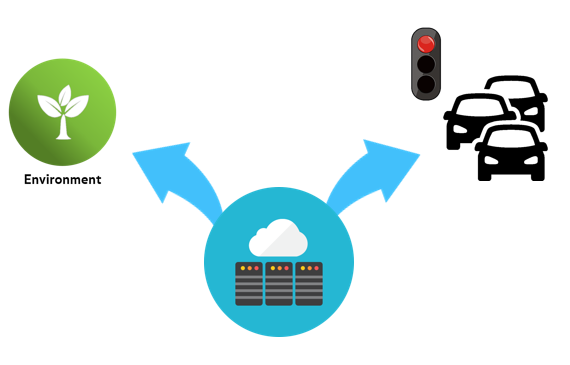
\includegraphics[width=1.0\textwidth]{pic1}
\caption[Trạm giám sát VOV Giao thông ]{Trạm giám sát VOV Giao thông}
\label{fig:pic1}
\end{figure}




\textbf{Bktraffic}  \url{http://traffic.hcmut.edu.vn} kết hợp hệ thống xe bus cùng với định vị GPS và gửi dữ liệu qua hạ tầng mạng 3G để theo dõi vị trí xe và tính toán tốc độ lưu thông trên đoạn đường xe đang lưu thông. Dự án này có hiệu quả cao vì hệ thống xe bus dày đặc và có thời gian hoạt động rộng. Tuy nhiên vẫn có những hạn chế như:
\begin{itemize}
\item[•]Vì chỉ giám sát trên xe bus nhưng nhiều trường hợp không hiệu quả khi áp dụng cho giao thông tại Việt Nam. Bởi vì đa số phương tiện giao thông ở Việt Nam là xe 2 bánh, do đó hệ thống bus di chuyển không phản ảnh được tình trạng lưu thông chung trên tuyến đường đó.
\item[•]Nhiều tuyến đường trên địa bàn thành phố mà xe bus vẫn chưa hoạt động, do vậy vẫn chưa có đủ dữ liệu cần thiết để.
\item[•]Mang tính phụ thuộc vào xe bus, vậy nên có sẽ có những trường hợp ảnh hưởng bởi hệ thống xe bus mà hệ thống sẽ không hoạt động hiệu quả được.
\end{itemize}

\begin{figure}[htbp!] 
\centering    
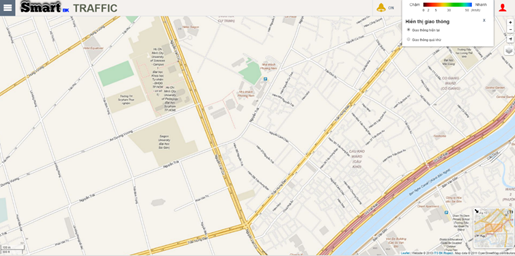
\includegraphics[width=1.0\textwidth]{pic2}
\caption[Ứng dụng Web SmartBKTraffic ]{ Ứng dụng Web SmartBKTraffic}
\label{fig:pic2}
\end{figure}




\textbf{Hệ thống quan trắc môi trường ở Hà Nội:} Thủ đô Hà Nội vừa lắp đặt hệ thống 80 trạm quan trắc. Hệ thống này có tính tương đồng với đề tài đang thực hiện. Tuy nhiên mục đích chính là để theo dõi môi trường sau sự cố bụi Thủy ngân và chưa thấy hướng ứng dụng vào hệ thống giao thông. Hơn nữa, các trạm này chiếm diện tích lắp đặt nên hạn chế khả năng triển khai số lượng lớn trên diện rộng.
\begin{figure}[htbp!] 
\centering    
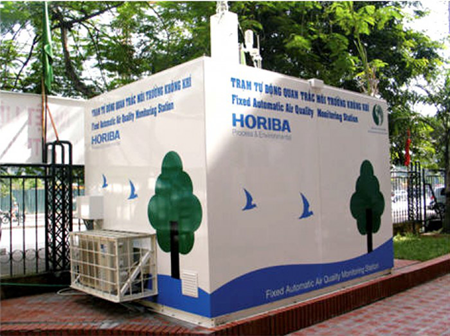
\includegraphics[width=1.0\textwidth]{pic3}
\caption[Trạm quan trắc môi trường tại Hà Nội ]{Trạm quan trắc môi trường tại Hà Nội}
\label{fig:pic3}
\end{figure}

\section{Các thiết bị phần cứng}
\subsection{Thiết bị thu thập dữ liệu}
Lorem ipsum dolor sit amet, consectetur adipiscing elit, sed do eiusmod tempor incididunt ut labore et dolore magna aliqua. Ut enim ad minim veniam, quis nostrud exercitation ullamco laboris nisi ut aliquip ex ea commodo consequat. Duis aute irure dolor in reprehenderit in voluptate velit esse cillum dolore eu fugiat nulla pariatur. Excepteur sint occaecat cupidatat non proident, sunt in culpa qui officia deserunt mollit anim id est laborum
\subsection{Các loại sensor}
Lorem ipsum dolor sit amet, consectetur adipiscing elit, sed do eiusmod tempor incididunt ut labore et dolore magna aliqua. Ut enim ad minim veniam, quis nostrud exercitation ullamco laboris nisi ut aliquip ex ea commodo consequat. Duis aute irure dolor in reprehenderit in voluptate velit esse cillum dolore eu fugiat nulla pariatur. Excepteur sint occaecat cupidatat non proident, sunt in culpa qui officia deserunt mollit anim id est laborum
\subsection{Mạch vi xử lý Arduino}
Lorem ipsum dolor sit amet, consectetur adipiscing elit, sed do eiusmod tempor incididunt ut labore et dolore magna aliqua. Ut enim ad minim veniam, quis nostrud exercitation ullamco laboris nisi ut aliquip ex ea commodo consequat. Duis aute irure dolor in reprehenderit in voluptate velit esse cillum dolore eu fugiat nulla pariatur. Excepteur sint occaecat cupidatat non proident, sunt in culpa qui officia deserunt mollit anim id est laborum
\subsection{Module SIM900}
Lorem ipsum dolor sit amet, consectetur adipiscing elit, sed do eiusmod tempor incididunt ut labore et dolore magna aliqua. Ut enim ad minim veniam, quis nostrud exercitation ullamco laboris nisi ut aliquip ex ea commodo consequat. Duis aute irure dolor in reprehenderit in voluptate velit esse cillum dolore eu fugiat nulla pariatur. Excepteur sint occaecat cupidatat non proident, sunt in culpa qui officia deserunt mollit anim id est laborum
\subsection{Năng lượng mặt trời}
Lorem ipsum dolor sit amet, consectetur adipiscing elit, sed do eiusmod tempor incididunt ut labore et dolore magna aliqua. Ut enim ad minim veniam, quis nostrud exercitation ullamco laboris nisi ut aliquip ex ea commodo consequat. Duis aute irure dolor in reprehenderit in voluptate velit esse cillum dolore eu fugiat nulla pariatur. Excepteur sint occaecat cupidatat non proident, sunt in culpa qui officia deserunt mollit anim id est laborum

\section{Kiến thức căn bản về ứng dụng web - di động và xây dựng Server}

\subsection{Giao thức TCP}
%TODO: ref https://vi.wikipedia.org/wiki/TCP
TCP (Transmission Control Protocol - "Giao thức điều khiển truyền vận") là một trong các giao thức cốt lõi của bộ giao thức TCP/IP. Sử dụng TCP, các ứng dụng trên các máy chủ được nối mạng có thể tạo các "kết nối" với nhau, mà qua đó chúng có thể trao đổi dữ liệu hoặc các gói tin. Giao thức này đảm bảo chuyển giao dữ liệu tới nơi nhận một cách đáng tin cậy và đúng thứ tự. TCP còn phân biệt giữa dữ liệu của nhiều ứng dụng (chẳng hạn, dịch vụ Web và dịch vụ thư điện tử) đồng thời chạy trên cùng một máy chủ.

TCP hỗ trợ nhiều giao thức ứng dụng phổ biến nhất trên Internet và các ứng dụng kết quả, trong đó có WWW, thư điện tử và Secure Shell.

Trong bộ giao thức TCP/IP, TCP là tầng trung gian giữa giao thức IP bên dưới và một ứng dụng bên trên. Các ứng dụng thường cần các kết nối đáng tin cậy kiểu đường ống để liên lạc với nhau, trong khi đó, giao thức IP không cung cấp những dòng kiểu đó, mà chỉ cung cấp dịch vụ chuyển gói tin không đáng tin cậy. TCP làm nhiệm vụ của tầng giao vận trong mô hình OSI đơn giản của các mạng máy tính.

Các ứng dụng gửi các dòng gồm các byte 8-bit tới TCP để chuyển qua mạng. TCP phân chia dòng byte này thành các đoạn (segment) có kích thước thích hợp (thường được quyết định dựa theo kích thước của đơn vị truyền dẫn tối đa (MTU) của tầng liên kết dữ liệu của mạng mà máy tính đang nằm trong đó). Sau đó, TCP chuyển các gói tin thu được tới giao thức IP để gửi nó qua một liên mạng tới mô đun TCP tại máy tính đích. TCP kiểm tra để đảm bảo không có gói tin nào bị thất lạc bằng cách gán cho mỗi gói tin một "số thứ tự" (sequence number). Số thứ tự này còn được sử dụng để đảm bảo dữ liệu được trao cho ứng dụng đích theo đúng thứ tự. Mô đun TCP tại đầu kia gửi lại "tin báo nhận" (acknowledgement) cho các gói tin đã nhận được thành công; một "đồng hồ" (timer) tại nơi gửi sẽ báo time-out nếu không nhận được tin báo nhận trong khoảng thời gian bằng một round-trip time (RTT), và dữ liệu (được coi là bị thất lạc) sẽ được gửi lại. TCP sử dụng checksum (giá trị kiểm tra) để xem có byte nào bị hỏng trong quá trình truyền hay không; giá trị này được tính toán cho mỗi khối dữ liệu tại nơi gửi trước khi nó được gửi, và được kiểm tra tại nơi nhận.

\subsection{Căn bản về RESTful Web services}

\textbf{Tổng quan về REST – Representational State Transfer}

REST là một kiểu kiến trúc dựa trên các tiêu chuẩn web và giao thức HTTP. REST được mô tả đầu tiên bởi Roy Fielding trong luận văn tiến sĩ của ông vào năm 2000.

Trong một kiến trúc REST thì tất cả mọi thứ là một nguồn tài nguyên. Một nguồn tài nguyên được truy cập thông qua một giao diện phổ biển dựa trên các phương pháp tiêu chuẩn HTTP.

Một kiến trúc REST thường có một REST server cung cấp truy cập đến các nguồn tài nguyên và một Rest client truy cập và trình sửa các tài nguyên đó.

REST cho phép các nguồn tài nguyên biểu diễn dưới nhiều kiểu khác nhau như Text, XML, JSON … Rest client có thể yêu cầu một kiểu biểu diễn cụ thể thông qua giao thức HTTP.

\textbf{Các phương thức HTTP}

Các phương thức PUT, GET, POST và DELETE thường được sử dụng trong kiến trúc REST

• \textbf{GET} định nghĩa một truy cập đọc nguồn tài nguyên mà không có tác dụng phụ. Nguồn tài nguyên không bao giờ thay đổi thông qua một yêu cầu GET.

• \textbf{PUT} dùng để tạo một tài nguyên mới.

• \textbf{DELETE} loại bỏ các nguồn tài nguyên.

• \textbf{POST} cập nhật một nguồn tài nguyên hiện có hoặc tạo ra một nguồn tài nguyên mới.

\textbf{RESTful webservice}

Một RESTful webservice được dựa trên các phương thức HTTP và các khái niệm về REST. Một RESTful webservice thường xác định URI cơ sở cho các dịch vụ, hỗ trợ các kiểu MIME (XML, Text, JSON,…) và tập các hoạt động (POST, GET, PUT, DELETE) đều được hỗ trợ.

\textbf{JSON (JavaScript Object Notation)}

Là một định dạng hoán vị dữ liệu nhanh. Chúng dễ dàng cho chúng ta đọc và viết. Dễ dàng cho thiết bị phân tích và phát sinh. Chúng là cơ sở dựa trên tập hợp của Ngôn Ngữ Lập Trình JavaScript, tiêu chuẩn ECMA-262 phiên bản 3 – tháng 12 năm 1999. JSON là một định dạng kiểu text mà hoàn toàn độc lập với các ngôn ngữ hoàn chỉnh, thuộc họ hàng với các ngôn ngữ họ hàng C, gồm có C, C++, C, Java, JavaScript, Perl, Python, và nhiều ngôn ngữ khác. Những đặc tính đó đã tạo nên JSON một ngôn ngữ hoán vị dữ liệu lý tưởng.

JSON được xây dựng trên 2 cấu trúc:

• Là tập hợp của các cặp tên và giá trịname – value. Trong những ngôn ngữ khác nhau, đây được nhận thấy như là một đối tượng (object), sự ghi (record), cấu trúc (struct), từ điển (dictionary), bảng băm (hash table), danh sách khóa (keyed list), hay mảng liên hợp.

• Là một tập hợp các giá trị đã được sắp xếp. Trong hầu hết các ngôn ngữ, nó được nhận thấy như là một mảng, vector, list hay là một dãy sequence.


\begin{figure}[H]
	\centering    
	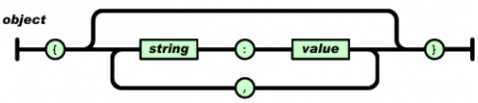
\includegraphics[width=1.0\textwidth]{json0}
	\caption[Cấu trúc của một đối tượng JSON]{Cấu trúc của một đối tượng JSON}
	\label{fig: json0}
\end{figure}

Một đối tượng là một tập hợp của các cặp tên/giá trị (name/value). Một đối tượng bắt đầu bởi dấu “{“ và kết thúc với dấu “}”. Từng tên được theo sau bởi dấu “:” và các cặp tên/giá trị được tách ra bởi dấu “,”.

\begin{figure}[H]
	\centering    
	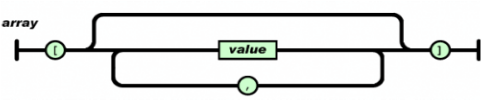
\includegraphics[width=1.0\textwidth]{json1}
	\caption[Cấu trúc mảng của JSON]{Cấu trúc mảng của JSON}
	\label{fig: json1}
\end{figure}

Một mảnglà một tập hợp các giá trị đã được xắp xếp, một mảng bắt đầu bởi dấu “[” và kết thúc với dấu “]”. Các giá trị được cách nhau bởi dấu “,”.
\begin{figure}[H]
	\centering    
	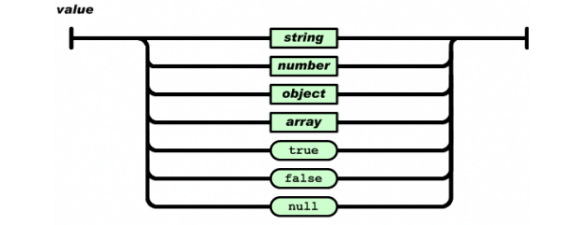
\includegraphics[width=1.0\textwidth]{json2}
	\caption[Cấu trúc của một đối tượng JSON]{Cấu trúc của một đối tượng JSON}
	\label{fig: json2}
\end{figure}

Một giá trị có thể là chuổi, số, đúng sai, hoặc là đối tượng hoặc mảng. Những cấu trúc này có thể được lồng vào nhau.

\textbf{JSON và Webservice}

Việc trao đổi thông tin, truyền tải dữ liệu giữa Webservice và ứng dụng người ta thường dùng XML hay JSON vì sự tiện nghi và cấu trúc dữ liệu nhỏ gọn của nó. JSON là một ngôn ngữ mới với tuổi đời con trẻ nhưng vẫn được ứng dụng nhiều bới những điểm lợi của nó:

• “Con người” có thể đọc được.

• Cú pháp gần với JavaScript nên rất dễ để sử dụng.

• Dữ liệu truyền tải ngắn gọn so với những định dạng dữ liệu như: XML, HTML…

• Việc phân tích (parse) dữ liệu từ dạng chuỗi (nhận từ server) sang dữ liệu có thể sử dụng được (thành Object, Number, Array) dễ dàng.
\begin{figure}[H]
	\centering    
	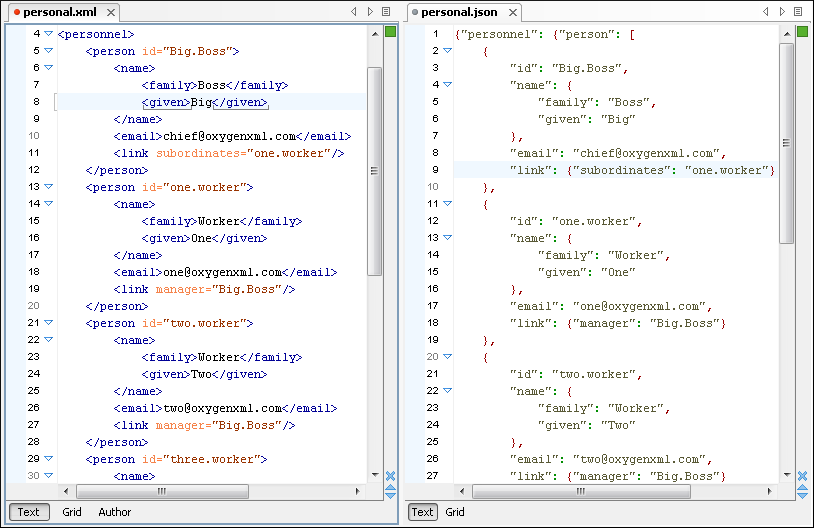
\includegraphics[width=1.0\textwidth]{json3}
	\caption[Cấu trúc mô tả XML-JSON]{Cấu trúc mô tả XML-JSON}
	\label{fig: json3}
\end{figure}
Nhằm mục đích giúp thời gian tương tác giữa người sử dụng với ứng dụng tiến gần đến thời gian thực, thì tốc độ được đặt lên hàng đầu, việc tăng tốc bằng cách “giảm tải” cũng là một giải pháp, chính vì vậy JSON được ưu ái hơn vì cú pháp ngắn gọn, đơn giản, tiết kiệm hơn XML.



\subsection{NodeJs}
%TODO: http://vietjack.com/nodejs/nodejs_la_gi.jsp
NodeJS là một nền tảng Server side được xây dựng dựa trên Javascript Engine (V8 Engine). Node.js được phát triển bởi Ryan Dahl năm 2009. Định nghĩa Nodejs bởi tài liệu chính thức : Node.js là một nền tảng dựa vào Chrome Javascript runtime để xây dựng các ứng dụng nhanh, có độ lớn. 

\begin{figure}[H]
	\centering    
	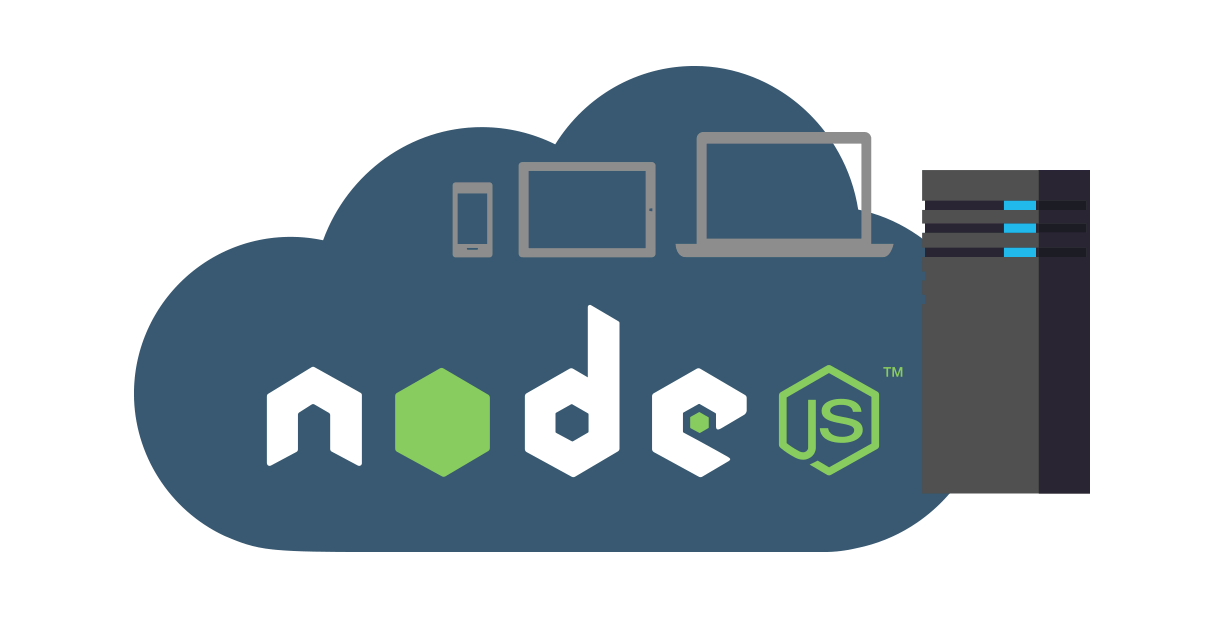
\includegraphics[width=1.0\textwidth]{nodejs0}
	\caption[Nền tảng Nodejs]{Nền tảng Nodejs}
	\label{fig: nodejs0}
\end{figure}

Node.js sử dụng các phần phát sinh các sự kiện (event-driven), mô hình non-blocking I/O để tạo ra các ứng dụng nhẹ và hiệu quả cho các ứng dụng về dữ liệu thời gian thực chạy trên các thiết bị phân tán.

\begin{figure}[H]
	\centering    
	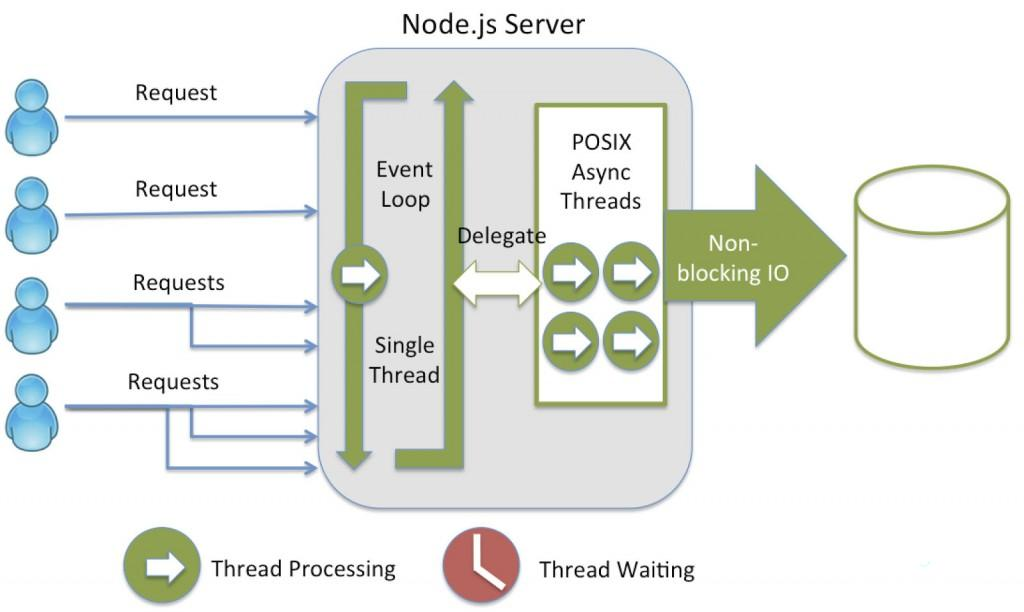
\includegraphics[width=1.0\textwidth]{nodejs1}
	\caption[Mô hình hoạt động Nodejs]{Mô hình hoạt động Nodejs}
	\label{fig: nodejs1}
\end{figure}

\subsection{Javascripts}
%TODO: ref https://vi.wikipedia.org/wiki/JavaScript
JavaScript, theo phiên bản hiện hành, là một ngôn ngữ lập trình kịch bản dựa trên đối tượng được phát triển từ các ý niệm nguyên mẫu. Ngôn ngữ này được dùng rộng rãi cho các trang web, nhưng cũng được dùng để tạo khả năng viết script sử dụng các đối tượng nằm sẵn trong các ứng dụng. Nó vốn được phát triển bởi Brendan Eich tại Hãng truyền thông Netscape với cái tên đầu tiên Mocha, rồi sau đó đổi tên thành LiveScript, và cuối cùng thành JavaScript. Giống Java, JavaScript có cú pháp tương tự C, nhưng nó gần với Self hơn Java. .js là phần mở rộng thường được dùng cho tập tin mã nguồn JavaScript.

%TODO: ref http://freetuts.net/javascript-la-gi-viet-ung-dung-javascript-dau-tien-263.html
Những ứng dụng to lớn của Javascript khiến người ta không thể quên nó được. Hiện nay có rất nhiều libraries, Framework được viêt như:

• AngularJS: Một thư viện dùng để xây dựng ứng dụng Single Page

• NodeJS: Một thư viện được phát triển phía Server dùng để xây dựng ứng dụng realtime

• Sencha Touch: Một Framework  dùng để xây dựng ứng dụng Mobile

• ExtJS: Một Framework dùng xây dựng ứng dụng quản lý (Web Applications)

• jQuery: Một thư viện rất mạnh về hiểu ứng

\subsection{Websocket - Socket.io}
%TODO: http://blog.rikkeisoft.com/seminar-gioi-thieu-ve-websocket-va-node-js/
WebSoket là công nghệ hỗ trợ giao tiếp hai chiều giữa client và server bằng cách sử dụng một TCP socket để tạo một kết nối hiệu quả và ít tốn kém. Mặc dù được thiết kế để chuyên sử dụng cho các ứng dụng web, lập trình viên vẫn có thể đưa chúng vào bất kì loại ứng dụng nào.
\begin{figure}[H]
	\centering    
	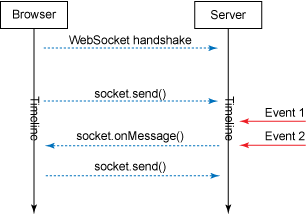
\includegraphics[width=0.5\textwidth]{websk}
	\caption[Mô hình hoạt động Websocket]{Mô hình hoạt động Websocket}
	\label{fig: websk}
\end{figure}

Kết nối được duy trì có thể viết và nhận dữ liệu bằng JavaScript như khi bạn đang sử dụng một TCP socket đơn thuần.

- HTTP: 871 x 10,000 = 8,710,000 bytes = 69,680,000 bits per second (66 Mbps)
- WebSocket: 2 x 10,000 = 20,000 bytes = 160,000 bits per second (0.153 Kbps)


\textbf{Socket.IO}

Socket.IO là một thư viện javascript có mục đích tạo ra các ứng dụng realtime trên trình duyệt cũng như thiết bị di động. Việc sử dụng thư viện này cũng rất đơn giản và giống nhau ở cả server lẫn client. 

\textbf{Tại sao Socket.IO ra đời?}

\begin{itemize}
\item[•]Javascript là ngôn ngữ lập trình hướng sự kiện, mà trong lập trình thời gian thực, cách tiếp cận bằng lập trình sự kiện là cách tiếp cận khôn ngoan nhất.
\item[•]Node.js chạy non-blocking việc hệ thống không phải tạm ngừng để xử lý xong một request sẽ giúp cho server trả lời client gần như ngay tức thì
\item[•]Lập trình socket yêu cầu bạn phải xây dựng được mô hình lắng nghe – trả lời từ cả 2 bên. Nói khác đi, vai trò của client và server phải tương đương nhau, mà client thì chạy bằng javascript, nên nếu server cũng chạy bằng javascript nữa, thì việc lập trình sẽ dễ dàng và thân thiện hơn.
\end{itemize}

Socket.IO hoạt động dựa trên các events tương tự như Websocket:

• \textbf{connect()}: kết nối với server socket

• \textbf{on(event\_name, listener)}: đăng kí lắng nghe sự kiện từ server trả về

• \textbf{emit(event\_name, data)}: gửi một sự kiện lên server

• \textbf{off(event\_name)}: ngừng lắng nghe một sự kiện nào đó

\subsection{RethinkDB}

\textbf{RethinkDB là gì?}

RethinkDB là một mã nguồn mở, dựa theo cấu trúc cơ sở dữ liệu NoSQL, tổ chức dữ liệu theo kiểu document-oriented database - một thiết kế riêng biệt cho việc lưu trữ document. Các cài đặt có thể là giả lập tương tác trên relational database, object database hay key-value store. Cơ sở dữ liệu được lưu trữ dưới dạng JSON  với các giản đồ động, và được thiết kế giúp hoạt động dễ dàng trong việc cập nhật và truy xuất dữ liệu theo thời gian thực với các ứng dụng. 

\begin{figure}[H]
	\centering    
	
\includegraphics[width=1\textwidth]{rethinkdb}
	\caption[Biểu tượng của RethinkDB]{Biểu tượng của RethinkDB}
	\label{fig: rethinkdb}
\end{figure}

RethinkDB sử dụng ngôn ngữ truy vấn ReQL được phát triển theo hướng đối tượng. Và ngôn ngữ này hỗ trợ cho các thao tác nhập bảng, quản lý nhóm, tích hợp và các hàm chức năng truy vấn cũng như event theo thời gian thực.

\begin{figure}[H]
	\centering    
	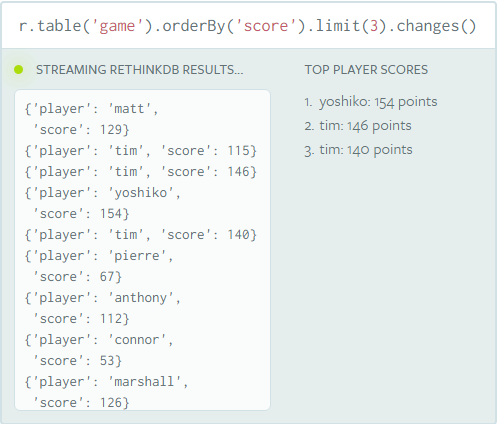
\includegraphics[width=0.9\textwidth]{rethink1}
	\caption[Đoạn code mẫu RethinkDB]{Đoạn code mẫu RethinkDB}
	\label{fig: rethink1}
\end{figure}

Như hình \ref{fig: rethink1} là ví dụ trực quan được demo trực tiếp tại trang chủ https://www.rethinkdb.com, có thể nhận thấy được cách thức khai báo và sử dụng RethinkDB:

• \textbf{r} : là đối tượng RethinkDB chúng ta khai báo trong ứng dụng.

• \textbf{table()} : là bảng giá trị đang truy vấn.

• \textbf{orderBy()} : hàm sắp xếp dữ liệu theo trường giá trị được khai báo.

• \textbf{limit()} : chọn ra những giá trị trong phạm vi được khai báo trong hàm.

• \textbf{changes()} : đây chính là đặc điểm khiến RethinkDB khác biệt so với các hệ quản lý dữ liệu khác. RethinkDB sẽ gọi hàm thực thi khi vùng giá trị truy vấn có thay dổi giá trị theo thời gian thật. không hoạt động theo cơ chế polling thường thấy ở các kiểu truy vấn dữ liệu khác.

%TODO: tham khảo tại https://vi.wikipedia.org/wiki/NoSQL
\subsection{Raspberry}

Raspbian là hệ điều hành mở và miễn phí được phát triển tối ưu hóa dựa trên nền Debian dành riêng cho thiết bị phần cứng Raspberry Pi. Hệ điều hành này bao gồm nhóm các chức năng và ứng dụng giúp Raspberry hoạt động. Hơn nữa, Raspbian cung cấp nhiều hơn là hệ điều hành thuần: hỗ trợ tới hơn 35,000 gói mở rộng và dễ dàng cài đặt trên Raspberry Pi. Raspbian ổn định và hiệu suất cao được hoàn thiện vào tháng 6 năm 2012. Tuy nhiên Raspbian vẫn đang được phát triển tới ngày nay và ngày càng cải thiện hiệu suất cũng như hỗ trợ các gói chức năng nhiều nhất có thể.
\begin{figure}[H]
	\centering    
	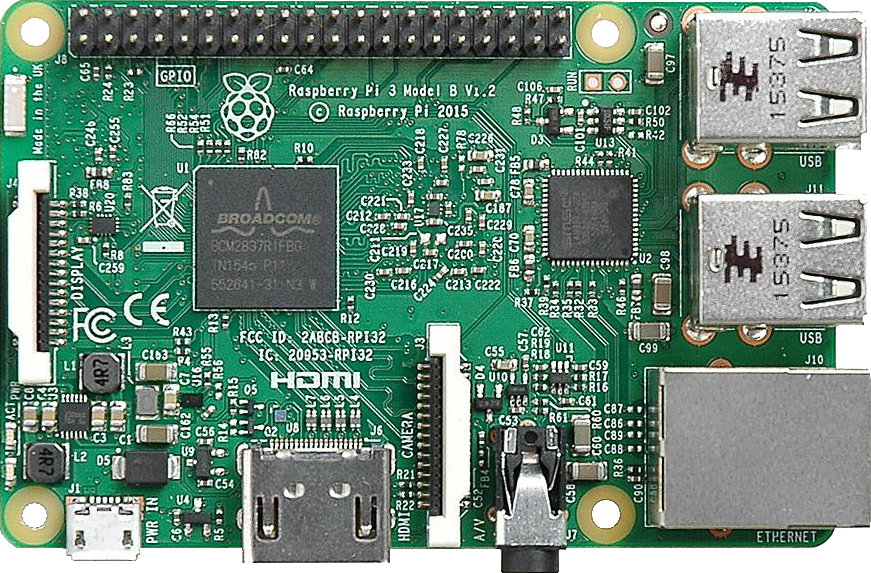
\includegraphics[width=0.9\textwidth]{rasp}
	\caption[Thiết bị Raspberry Pi]{Thiết bị Raspberry Pi}
	\label{fig: rasp}
\end{figure}

Vì sao lựa chọn Raspberry:

• Là một máy tính độc lập chạy trên nền tảng Linux, điều này làm cho việc chạy các ứng dụng Nodejs hay RethinkDB hoạt động được trên Raspberry Pi.

• Hiệu suất đáp ứng nhu cầu làm server của đề tài yêu cầu với mức độ tiêu thụ năng lượng cực kì ít.

\subsection{Framework Ionic}
Lorem ipsum dolor sit amet, consectetur adipiscing elit, sed do eiusmod tempor incididunt ut labore et dolore magna aliqua. Ut enim ad minim veniam, quis nostrud exercitation ullamco laboris nisi ut aliquip ex ea commodo consequat. Duis aute irure dolor in reprehenderit in voluptate velit esse cillum dolore eu fugiat nulla pariatur. Excepteur sint occaecat cupidatat non proident, sunt in culpa qui officia deserunt mollit anim id est laborum
% **************************** Define Graphics Path **************************
\ifpdf
\graphicspath{{Chapter3/Figs/Raster/}{Chapter3/Figs/PDF/}{Chapter3/Figs/}}
\else
\graphicspath{{Chapter3/Figs/Vector/}{Chapter3/Figs/}}
\fi

\chapter{Thiết kế và Hiện thực}

\section{Thiết kế hệ thống}
\subsection{Kiến trúc mô hình hệ thống}
Lorem ipsum dolor sit amet, consectetur adipiscing elit, sed do eiusmod tempor incididunt ut labore et dolore magna aliqua. Ut enim ad minim veniam, quis nostrud exercitation ullamco laboris nisi ut aliquip ex ea commodo consequat. Duis aute irure dolor in reprehenderit in voluptate velit esse cillum dolore eu fugiat nulla pariatur. Excepteur sint occaecat cupidatat non proident, sunt in culpa qui officia deserunt mollit anim id est laborum
\subsection{Các ràng buộc của hệ thống}
Lorem ipsum dolor sit amet, consectetur adipiscing elit, sed do eiusmod tempor incididunt ut labore et dolore magna aliqua. Ut enim ad minim veniam, quis nostrud exercitation ullamco laboris nisi ut aliquip ex ea commodo consequat. Duis aute irure dolor in reprehenderit in voluptate velit esse cillum dolore eu fugiat nulla pariatur. Excepteur sint occaecat cupidatat non proident, sunt in culpa qui officia deserunt mollit anim id est laborum
\subsection{Mô hình ứng dụng trình bày dữ liệu}
Lorem ipsum dolor sit amet, consectetur adipiscing elit, sed do eiusmod tempor incididunt ut labore et dolore magna aliqua. Ut enim ad minim veniam, quis nostrud exercitation ullamco laboris nisi ut aliquip ex ea commodo consequat. Duis aute irure dolor in reprehenderit in voluptate velit esse cillum dolore eu fugiat nulla pariatur. Excepteur sint occaecat cupidatat non proident, sunt in culpa qui officia deserunt mollit anim id est laborum
\section{Hiện thực Node cảm biến}
\subsection{Các node cảm biến thu thập dữ liệu}
Lorem ipsum dolor sit amet, consectetur adipiscing elit, sed do eiusmod tempor incididunt ut labore et dolore magna aliqua. Ut enim ad minim veniam, quis nostrud exercitation ullamco laboris nisi ut aliquip ex ea commodo consequat. Duis aute irure dolor in reprehenderit in voluptate velit esse cillum dolore eu fugiat nulla pariatur. Excepteur sint occaecat cupidatat non proident, sunt in culpa qui officia deserunt mollit anim id est laborum
\subsection{Ứng dụng theo dõi dữ liệu và đánh giá}
Lorem ipsum dolor sit amet, consectetur adipiscing elit, sed do eiusmod tempor incididunt ut labore et dolore magna aliqua. Ut enim ad minim veniam, quis nostrud exercitation ullamco laboris nisi ut aliquip ex ea commodo consequat. Duis aute irure dolor in reprehenderit in voluptate velit esse cillum dolore eu fugiat nulla pariatur. Excepteur sint occaecat cupidatat non proident, sunt in culpa qui officia deserunt mollit anim id est laborum
\section{Hệ thống Server lưu trữ dữ liệu và cung cấp API}
Lorem ipsum dolor sit amet, consectetur adipiscing elit, sed do eiusmod tempor incididunt ut labore et dolore magna aliqua. Ut enim ad minim veniam, quis nostrud exercitation ullamco laboris nisi ut aliquip ex ea commodo consequat. Duis aute irure dolor in reprehenderit in voluptate velit esse cillum dolore eu fugiat nulla pariatur. Excepteur sint occaecat cupidatat non proident, sunt in culpa qui officia deserunt mollit anim id est laborum
\subsection{Cấu trúc tổ chức tập tin}
Lorem ipsum dolor sit amet, consectetur adipiscing elit, sed do eiusmod tempor incididunt ut labore et dolore magna aliqua. Ut enim ad minim veniam, quis nostrud exercitation ullamco laboris nisi ut aliquip ex ea commodo consequat. Duis aute irure dolor in reprehenderit in voluptate velit esse cillum dolore eu fugiat nulla pariatur. Excepteur sint occaecat cupidatat non proident, sunt in culpa qui officia deserunt mollit anim id est laborum
\subsection{Thiết kế API}
Lorem ipsum dolor sit amet, consectetur adipiscing elit, sed do eiusmod tempor incididunt ut labore et dolore magna aliqua. Ut enim ad minim veniam, quis nostrud exercitation ullamco laboris nisi ut aliquip ex ea commodo consequat. Duis aute irure dolor in reprehenderit in voluptate velit esse cillum dolore eu fugiat nulla pariatur. Excepteur sint occaecat cupidatat non proident, sunt in culpa qui officia deserunt mollit anim id est laborum

	\begin{lstlisting}[caption=My Javascript Example]
	Name.prototype = {
	methodName: function(params){
	var doubleQuoteString = "some text";
	var singleQuoteString = 'some more text';
	// this is a comment
	if(this.confirmed != null && typeof(this.confirmed) == Boolean && this.confirmed == true){
	document.createElement('h3');
	$('#system').append("This looks great");
	return false;
	} else {
	throw new Error;
	}
	}
	}
	\end{lstlisting}
\subsection{Xây dựng Web Server}
Lorem ipsum dolor sit amet, consectetur adipiscing elit, sed do eiusmod tempor incididunt ut labore et dolore magna aliqua. Ut enim ad minim veniam, quis nostrud exercitation ullamco laboris nisi ut aliquip ex ea commodo consequat. Duis aute irure dolor in reprehenderit in voluptate velit esse cillum dolore eu fugiat nulla pariatur. Excepteur sint occaecat cupidatat non proident, sunt in culpa qui officia deserunt mollit anim id est laborum
\section{Ứng dụng thiết bị di động}
Lorem ipsum dolor sit amet, consectetur adipiscing elit, sed do eiusmod tempor incididunt ut labore et dolore magna aliqua. Ut enim ad minim veniam, quis nostrud exercitation ullamco laboris nisi ut aliquip ex ea commodo consequat. Duis aute irure dolor in reprehenderit in voluptate velit esse cillum dolore eu fugiat nulla pariatur. Excepteur sint occaecat cupidatat non proident, sunt in culpa qui officia deserunt mollit anim id est laborum
\chapter{Kết quả thực nhiệm và Đánh giá}

% **************************** Define Graphics Path **************************
\ifpdf
    \graphicspath{{Chapter4/Figs/Raster/}{Chapter4/Figs/PDF/}{Chapter4/Figs/}}
\else
    \graphicspath{{Chapter4/Figs/Vector/}{Chapter4/Figs/}}
\fi

\section{Mức độ tiêu hao năng}
\textbf{nói về đo đạc v.v chỗ này nên bỏ bên hiện thực hay kết quả ?}

Lorem ipsum dolor sit amet, consectetur adipiscing elit, sed do eiusmod tempor incididunt ut labore et dolore magna aliqua. Ut enim ad minim veniam, quis nostrud exercitation ullamco laboris nisi ut aliquip ex ea commodo consequat. Duis aute irure dolor in reprehenderit in voluptate velit esse cillum dolore eu fugiat nulla pariatur. Excepteur sint occaecat cupidatat non proident, sunt in culpa qui officia deserunt mollit anim id est laborum
\section{Tính ổn định của node cảm biến}
\textbf{này nói về mấy tháng đo, gió mưa đồ}

Lorem ipsum dolor sit amet, consectetur adipiscing elit, sed do eiusmod tempor incididunt ut labore et dolore magna aliqua. Ut enim ad minim veniam, quis nostrud exercitation ullamco laboris nisi ut aliquip ex ea commodo consequat. Duis aute irure dolor in reprehenderit in voluptate velit esse cillum dolore eu fugiat nulla pariatur. Excepteur sint occaecat cupidatat non proident, sunt in culpa qui officia deserunt mollit anim id est laborum
\section{Tính ổn định của Server}
\textbf{Nói về thời gian đáp ứng truyền nhận dữ liệu}

Lorem ipsum dolor sit amet, consectetur adipiscing elit, sed do eiusmod tempor incididunt ut labore et dolore magna aliqua. Ut enim ad minim veniam, quis nostrud exercitation ullamco laboris nisi ut aliquip ex ea commodo consequat. Duis aute irure dolor in reprehenderit in voluptate velit esse cillum dolore eu fugiat nulla pariatur. Excepteur sint occaecat cupidatat non proident, sunt in culpa qui officia deserunt mollit anim id est laborum
\section{Đánh giá lập trình ứng dụng Mobile sử dụng APIs}

Lorem ipsum dolor sit amet, consectetur adipiscing elit, sed do eiusmod tempor incididunt ut labore et dolore magna aliqua. Ut enim ad minim veniam, quis nostrud exercitation ullamco laboris nisi ut aliquip ex ea commodo consequat. Duis aute irure dolor in reprehenderit in voluptate velit esse cillum dolore eu fugiat nulla pariatur. Excepteur sint occaecat cupidatat non proident, sunt in culpa qui officia deserunt mollit anim id est laborum

\chapter{Tổng kết và Hướng phát triển cho tương lai}

% **************************** Define Graphics Path **************************
\ifpdf
    \graphicspath{{Chapter5/Figs/Raster/}{Chapter5/Figs/PDF/}{Chapter5/Figs/}}
\else
    \graphicspath{{Chapter5/Figs/Vector/}{Chapter5/Figs/}}
\fi

\section{Tổng kết}
\subsection{Những gì đạt được}
Lorem ipsum dolor sit amet, consectetur adipiscing elit, sed do eiusmod tempor incididunt ut labore et dolore magna aliqua. Ut enim ad minim veniam, quis nostrud exercitation ullamco laboris nisi ut aliquip ex ea commodo consequat. Duis aute irure dolor in reprehenderit in voluptate velit esse cillum dolore eu fugiat nulla pariatur. Excepteur sint occaecat cupidatat non proident, sunt in culpa qui officia deserunt mollit anim id est laborum
\subsection{Những khó khăn và hạn chế}
Lorem ipsum dolor sit amet, consectetur adipiscing elit, sed do eiusmod tempor incididunt ut labore et dolore magna aliqua. Ut enim ad minim veniam, quis nostrud exercitation ullamco laboris nisi ut aliquip ex ea commodo consequat. Duis aute irure dolor in reprehenderit in voluptate velit esse cillum dolore eu fugiat nulla pariatur. Excepteur sint occaecat cupidatat non proident, sunt in culpa qui officia deserunt mollit anim id est laborum
And now I begin my third chapter here \dots
\section{Hướng phát triển tương lai}
Lorem ipsum dolor sit amet, consectetur adipiscing elit, sed do eiusmod tempor incididunt ut labore et dolore magna aliqua. Ut enim ad minim veniam, quis nostrud exercitation ullamco laboris nisi ut aliquip ex ea commodo consequat. Duis aute irure dolor in reprehenderit in voluptate velit esse cillum dolore eu fugiat nulla pariatur. Excepteur sint occaecat cupidatat non proident, sunt in culpa qui officia deserunt mollit anim id est laborum
%\include{Chapter6/chapter6}
%\include{Chapter7/chapter7}



% ********************************** Back Matter *******************************
% Backmatter should be commented out, if you are using appendices after References
%\backmatter

% ********************************** Bibliography ******************************
\begin{spacing}{0.9}

% To use the conventional natbib style referencing
% Bibliography style previews: http://nodonn.tipido.net/bibstyle.php
% Reference styles: http://sites.stat.psu.edu/~surajit/present/bib.htm

\bibliographystyle{apalike}
%\bibliographystyle{unsrt} % Use for unsorted references  
%\bibliographystyle{plainnat} % use this to have URLs listed in References
\cleardoublepage
\bibliography{References/references} % Path to your References.bib file


% If you would like to use BibLaTeX for your references, pass `custombib' as
% an option in the document class. The location of 'reference.bib' should be
% specified in the preamble.tex file in the custombib section.
% Comment out the lines related to natbib above and uncomment the following line.

%\printbibliography[heading=bibintoc, title={References}]


\end{spacing}

%\appendix
%% ******************************* Thesis Appendix A ****************************
\chapter{How to install \LaTeX} 

\section*{Windows OS}

\subsection*{TeXLive package - full version}
\begin{enumerate}
\item	Download the TeXLive ISO (2.2GB) from\\
\href{https://www.tug.org/texlive/}{https://www.tug.org/texlive/}
\item	Download WinCDEmu (if you don't have a virtual drive) from \\
\href{http://wincdemu.sysprogs.org/download/}
{http://wincdemu.sysprogs.org/download/}
\item	To install Windows CD Emulator follow the instructions at\\
\href{http://wincdemu.sysprogs.org/tutorials/install/}
{http://wincdemu.sysprogs.org/tutorials/install/}
\item	Right click the iso and mount it using the WinCDEmu as shown in \\
\href{http://wincdemu.sysprogs.org/tutorials/mount/}{
http://wincdemu.sysprogs.org/tutorials/mount/}
\item	Open your virtual drive and run setup.pl
\end{enumerate}

or

\subsection*{Basic MikTeX - \TeX~ distribution}
\begin{enumerate}
\item	Download Basic-MiK\TeX (32bit or 64bit) from\\
\href{http://miktex.org/download}{http://miktex.org/download}
\item	Run the installer 
\item	To add a new package go to Start >> All Programs >> MikTex >> Maintenance (Admin) and choose Package Manager
\item	Select or search for packages to install
\end{enumerate}

\subsection*{TexStudio - \TeX~ editor}
\begin{enumerate}
\item	Download TexStudio from\\
\href{http://texstudio.sourceforge.net/\#downloads}
{http://texstudio.sourceforge.net/\#downloads} 
\item	Run the installer
\end{enumerate}

\section*{Mac OS X}
\subsection*{MacTeX - \TeX~ distribution}
\begin{enumerate}
\item	Download the file from\\
\href{https://www.tug.org/mactex/}{https://www.tug.org/mactex/}
\item	Extract and double click to run the installer. It does the entire configuration, sit back and relax.
\end{enumerate}

\subsection*{TexStudio - \TeX~ editor}
\begin{enumerate}
\item	Download TexStudio from\\
\href{http://texstudio.sourceforge.net/\#downloads}
{http://texstudio.sourceforge.net/\#downloads} 
\item	Extract and Start
\end{enumerate}


\section*{Unix/Linux}
\subsection*{TeXLive - \TeX~ distribution}
\subsubsection*{Getting the distribution:}
\begin{enumerate}
\item	TexLive can be downloaded from\\
\href{http://www.tug.org/texlive/acquire-netinstall.html}
{http://www.tug.org/texlive/acquire-netinstall.html}.
\item	TexLive is provided by most operating system you can use (rpm,apt-get or yum) to get TexLive distributions
\end{enumerate}

\subsubsection*{Installation}
\begin{enumerate}
\item	Mount the ISO file in the mnt directory
\begin{verbatim}
mount -t iso9660 -o ro,loop,noauto /your/texlive####.iso /mnt
\end{verbatim}

\item	Install wget on your OS (use rpm, apt-get or yum install)
\item	Run the installer script install-tl.
\begin{verbatim}
	cd /your/download/directory
	./install-tl
\end{verbatim}
\item	Enter command `i' for installation

\item	Post-Installation configuration:\\
\href{http://www.tug.org/texlive/doc/texlive-en/texlive-en.html\#x1-320003.4.1}
{http://www.tug.org/texlive/doc/texlive-en/texlive-en.html\#x1-320003.4.1} 
\item	Set the path for the directory of TexLive binaries in your .bashrc file
\end{enumerate}

\subsubsection*{For 32bit OS}
For Bourne-compatible shells such as bash, and using Intel x86 GNU/Linux and a default directory setup as an example, the file to edit might be \begin{verbatim}
edit $~/.bashrc file and add following lines
PATH=/usr/local/texlive/2011/bin/i386-linux:$PATH; 
export PATH 
MANPATH=/usr/local/texlive/2011/texmf/doc/man:$MANPATH;
export MANPATH 
INFOPATH=/usr/local/texlive/2011/texmf/doc/info:$INFOPATH;
export INFOPATH
\end{verbatim}
\subsubsection*{For 64bit OS}
\begin{verbatim}
edit $~/.bashrc file and add following lines
PATH=/usr/local/texlive/2011/bin/x86_64-linux:$PATH;
export PATH 
MANPATH=/usr/local/texlive/2011/texmf/doc/man:$MANPATH;
export MANPATH 
INFOPATH=/usr/local/texlive/2011/texmf/doc/info:$INFOPATH;
export INFOPATH

\end{verbatim}



%\subsection{Installing directly using Linux packages} 
\subsubsection*{Fedora/RedHat/CentOS:}
\begin{verbatim} 
sudo yum install texlive 
sudo yum install psutils 
\end{verbatim}


\subsubsection*{SUSE:}
\begin{verbatim}
sudo zypper install texlive
\end{verbatim}


\subsubsection*{Debian/Ubuntu:}
\begin{verbatim} 
sudo apt-get install texlive texlive-latex-extra 
sudo apt-get install psutils
\end{verbatim}

% ********************************** Appendices ********************************

\begin{appendices} % Using appendices environment for more functunality

%% ******************************* Thesis Appendix A ****************************
\chapter{How to install \LaTeX} 

\section*{Windows OS}

\subsection*{TeXLive package - full version}
\begin{enumerate}
\item	Download the TeXLive ISO (2.2GB) from\\
\href{https://www.tug.org/texlive/}{https://www.tug.org/texlive/}
\item	Download WinCDEmu (if you don't have a virtual drive) from \\
\href{http://wincdemu.sysprogs.org/download/}
{http://wincdemu.sysprogs.org/download/}
\item	To install Windows CD Emulator follow the instructions at\\
\href{http://wincdemu.sysprogs.org/tutorials/install/}
{http://wincdemu.sysprogs.org/tutorials/install/}
\item	Right click the iso and mount it using the WinCDEmu as shown in \\
\href{http://wincdemu.sysprogs.org/tutorials/mount/}{
http://wincdemu.sysprogs.org/tutorials/mount/}
\item	Open your virtual drive and run setup.pl
\end{enumerate}

or

\subsection*{Basic MikTeX - \TeX~ distribution}
\begin{enumerate}
\item	Download Basic-MiK\TeX (32bit or 64bit) from\\
\href{http://miktex.org/download}{http://miktex.org/download}
\item	Run the installer 
\item	To add a new package go to Start >> All Programs >> MikTex >> Maintenance (Admin) and choose Package Manager
\item	Select or search for packages to install
\end{enumerate}

\subsection*{TexStudio - \TeX~ editor}
\begin{enumerate}
\item	Download TexStudio from\\
\href{http://texstudio.sourceforge.net/\#downloads}
{http://texstudio.sourceforge.net/\#downloads} 
\item	Run the installer
\end{enumerate}

\section*{Mac OS X}
\subsection*{MacTeX - \TeX~ distribution}
\begin{enumerate}
\item	Download the file from\\
\href{https://www.tug.org/mactex/}{https://www.tug.org/mactex/}
\item	Extract and double click to run the installer. It does the entire configuration, sit back and relax.
\end{enumerate}

\subsection*{TexStudio - \TeX~ editor}
\begin{enumerate}
\item	Download TexStudio from\\
\href{http://texstudio.sourceforge.net/\#downloads}
{http://texstudio.sourceforge.net/\#downloads} 
\item	Extract and Start
\end{enumerate}


\section*{Unix/Linux}
\subsection*{TeXLive - \TeX~ distribution}
\subsubsection*{Getting the distribution:}
\begin{enumerate}
\item	TexLive can be downloaded from\\
\href{http://www.tug.org/texlive/acquire-netinstall.html}
{http://www.tug.org/texlive/acquire-netinstall.html}.
\item	TexLive is provided by most operating system you can use (rpm,apt-get or yum) to get TexLive distributions
\end{enumerate}

\subsubsection*{Installation}
\begin{enumerate}
\item	Mount the ISO file in the mnt directory
\begin{verbatim}
mount -t iso9660 -o ro,loop,noauto /your/texlive####.iso /mnt
\end{verbatim}

\item	Install wget on your OS (use rpm, apt-get or yum install)
\item	Run the installer script install-tl.
\begin{verbatim}
	cd /your/download/directory
	./install-tl
\end{verbatim}
\item	Enter command `i' for installation

\item	Post-Installation configuration:\\
\href{http://www.tug.org/texlive/doc/texlive-en/texlive-en.html\#x1-320003.4.1}
{http://www.tug.org/texlive/doc/texlive-en/texlive-en.html\#x1-320003.4.1} 
\item	Set the path for the directory of TexLive binaries in your .bashrc file
\end{enumerate}

\subsubsection*{For 32bit OS}
For Bourne-compatible shells such as bash, and using Intel x86 GNU/Linux and a default directory setup as an example, the file to edit might be \begin{verbatim}
edit $~/.bashrc file and add following lines
PATH=/usr/local/texlive/2011/bin/i386-linux:$PATH; 
export PATH 
MANPATH=/usr/local/texlive/2011/texmf/doc/man:$MANPATH;
export MANPATH 
INFOPATH=/usr/local/texlive/2011/texmf/doc/info:$INFOPATH;
export INFOPATH
\end{verbatim}
\subsubsection*{For 64bit OS}
\begin{verbatim}
edit $~/.bashrc file and add following lines
PATH=/usr/local/texlive/2011/bin/x86_64-linux:$PATH;
export PATH 
MANPATH=/usr/local/texlive/2011/texmf/doc/man:$MANPATH;
export MANPATH 
INFOPATH=/usr/local/texlive/2011/texmf/doc/info:$INFOPATH;
export INFOPATH

\end{verbatim}



%\subsection{Installing directly using Linux packages} 
\subsubsection*{Fedora/RedHat/CentOS:}
\begin{verbatim} 
sudo yum install texlive 
sudo yum install psutils 
\end{verbatim}


\subsubsection*{SUSE:}
\begin{verbatim}
sudo zypper install texlive
\end{verbatim}


\subsubsection*{Debian/Ubuntu:}
\begin{verbatim} 
sudo apt-get install texlive texlive-latex-extra 
sudo apt-get install psutils
\end{verbatim}

%% ******************************* Thesis Appendix B ********************************

\chapter{Installing the CUED class file}

\LaTeX.cls files can be accessed system-wide when they are placed in the
<texmf>/tex/latex directory, where <texmf> is the root directory of the user’s \TeX installation. On systems that have a local texmf tree (<texmflocal>), which
may be named ``texmf-local'' or ``localtexmf'', it may be advisable to install packages in <texmflocal>, rather than <texmf> as the contents of the former, unlike that of the latter, are preserved after the \LaTeX system is reinstalled and/or upgraded.

It is recommended that the user create a subdirectory <texmf>/tex/latex/CUED for all CUED related \LaTeX class and package files. On some \LaTeX systems, the directory look-up tables will need to be refreshed after making additions or deletions to the system files. For \TeX Live systems this is accomplished via executing ``texhash'' as root. MIK\TeX users can run ``initexmf -u'' to accomplish the same thing.

Users not willing or able to install the files system-wide can install them in their personal directories, but will then have to provide the path (full or relative) in addition to the filename when referring to them in \LaTeX.



\end{appendices}

% *************************************** Index ********************************
\printthesisindex % If index is present

\end{document}
